\documentclass[11pt]{book}

\usepackage{times}

\usepackage{amsmath}
\usepackage{bm}
\usepackage{graphicx}
\usepackage{tikz-cd}
\usepackage{amsfonts}
\usepackage{geometry}
\def\ii{{\rm i}}
\def\dd{{\rm d}}

\newcommand{\re}[1]{\textcolor{blue}{[{\bf RE}: #1]}}
\newcommand{\cl}[1]{\textcolor{cyan}{[{\bf CL}: #1]}}

\setlength{\oddsidemargin}{1.5cm}
\setlength{\evensidemargin}{0cm}
\setlength{\topmargin}{1mm}
\setlength{\headheight}{1.36cm}
\setlength{\headsep}{1.00cm}
\setlength{\textheight}{19cm}
\setlength{\textwidth}{14.5cm}
\setlength{\marginparsep}{1mm}
\setlength{\marginparwidth}{3cm}
\setlength{\footskip}{2.36cm}

\DeclareMathOperator{\Li}{Li}
\DeclareMathOperator{\diag}{diag}
\DeclareMathOperator{\Arctan}{Arctan}
\DeclareMathOperator*{\argmax}{arg\,max}

\begin{document}

\pagestyle{empty}
\begin{center}
\vspace{1cm}
{\Huge Oscillon Dynamics in\\Classical Scalar Field Theory}\\
\vspace{35mm} 

\includegraphics[width=2cm]{logo.jpg}\\
\vspace{45mm}
{\Large Chang Liu}\\
\vspace{1ex}
Department of Physics\\
The University of Auckland\\
\vspace{5ex}
Supervisor: Prof.~Richard Easther\\
\vspace*{30mm}
A thesis submitted in partial fulfillment of the requirements for the degree of Master of Science in Physics, The University of Auckland, 2017.
\end{center}

\newpage

\chapter*{Abstract}       
Oscillons are spatially compact, temporally oscillatory, {\em long-lived} solutions to a non-linear wave equation. In this Thesis, we review the literature from both applied mathematics and physics on the subject of oscillon dynamics, and point out that the existing method of studying oscillon properties is not applicable to axion-monodromy oscillons, the understanding of which comprises the main goal of this project.

Using the exact integrability of the 1D sine-Gordon equation, we construct an exact oscillon solution with two independent time-scales, named the ``two-scale'' solution, and numerically extend it to more general potentials and dimensionalities. We show that the novel field dynamics, namely the breathing modes and off-center peaks, is present in more general settings by proposing three numerical metrics capturing the essential field dynamics.

Finally, we apply the exact two-scale solution to the axion-monodromy oscillons, in the setting of a post-inflationary universe, and conclude that the analytic ansatz obtained from the exact solution can account for local, but not global, breathing dynamics of the axion-monodromy oscillons in the very early universe.

\setcounter{page}{1}
\pagestyle{headings}

\addcontentsline{toc}{chapter}{Abstract}

\chapter*{Acknowledgements}

I would like to thank my supervisor, Prof.~Richard Easther, for guidance and support. Additionally, the following people have contributed to the project (through useful discussions): Mustafa Amin, Ed Copeland, Miro Erkintalo, Eugene Lim, Joshua Rippon, and Bonnie Yu. In particular, Mustafa Amin and Joshua Rippon created the numerical code used in part of the project.
\medbreak
I would like to thank the New Zealand eScience Infrastructure (NeSI) high-performance computing centre, in particular, Dr.~Sina Masoud-Ansari and Dr.~Chris Scott, for computational resources and support.
\medbreak
Lastly, love and peace to Mr.~Steal Your Curls (and crew). Hoost.

\setcounter{secnumdepth}{3} % organisational level that receives a numbers
\setcounter{tocdepth}{3}    % print table of contents for level 3
\tableofcontents            % print the table of contents

\chapter{Introduction}
\section{Overview of the Thesis}
In this Thesis, we present the studies done in a year-long Master of Science project investigating the dynamics of oscillons in classical scalar field theories. In particular, the study is focused on the dynamics of 3D axion-monodromy oscillons in the setting of a (p)re-heating universe, towards the end of the inflationary stage.

The outline of the Thesis is as follows: We first review the literature from both applied mathematics and physics. We then point out the limitations of previous studies when applied to axion-monodromy oscillons. This is the motivation for a more complex oscillon solution, which is main contribution of this Thesis: a novel, two-scale oscillon solution. Using the exact integrability of the 1D sine-Gordon equation, we will construct an exact oscillon solution with two independent time-scales, and numerically extend it to more general potentials and dimensionalities. We will conclude that the novel field dynamics, namely the breathing modes and off-center peaks of the exact solution, is still present in the more general settings.

Finally, we will apply our results on the two-scale solution to the axion-monodromy oscillons, in the setting of a post-inflationary universe, and conclude that the analytic ansatz obtained from the exact two-scale solution can account for local, but not global, breathing dynamics of the axion-monodromy oscillons in the early-universe.

\section{What is an oscillon?}
An oscillon is a spatially compact, temporally oscillatory, {\em long-lived} solution to a non-linear wave equation. Mathematically speaking, given the standard wave equation in $d=1+D$ dimensions\footnote{In this thesis, we take the metric signature to be $\eta^{\mu\nu} = \diag(+1,-1,\ldots,-1)$}
\begin{equation}\label{wave}
  Du := \partial^2 u + V'(u) = 0
\end{equation}
with a non-linear potential $V(u)$, we define an oscillon solution to be a $C^\infty$ function that satisfies the following conditions:
\begin{enumerate}
\item For all fixed times $t$, the functions $u(t, x^i)$ have compact support along the spatial dimensions, such that the total energy of the oscillon
  \begin{equation}
    \rho = \int \left[\frac{1}{2}\left(u_t^2+ \nabla u\cdot \nabla u \right) + V(u) - V(0)\right] \dd^D x
  \end{equation}
  is finite for all time.
\item For all fixed points $x^i$, the functions $u(t, x^i)$ are quasi-oscillatory and bounded in time, with long but typically finite lifetime.
\end{enumerate}

Typically, $u(t,x^i)$ solves the non-linear wave equation (\ref{wave}) with a small radiation residual: $Du(t,x^i) \approx 0$. At large distances there will be a clear distinction between the outgoing radiation and the oscillon. Near ``edge of the oscillon'', the distinction will be less clear.

Intuitively speaking, an oscillon is a spatially localized ``lump'' of mass-energy that oscillates around $u=0$ (see Fig.~\ref{nntliquid}), which is presumptively a (local) minimum of the potential. What makes oscillons interesting from a physical perspective is that for many non-linear potentials, oscillons are meta-stable: that is, although an oscillon solution contains outward radiations and will eventually decay, the time it takes to do so is significantly longer than the fundamental oscillation time-scale. For the special case of the sine-Gordon potential in one spatial dimension, oscillon solutions are exact and do not decay at all. This meta-stability makes oscillon solutions interesting in a wide range of physics phenomena.

\begin{figure}\centering
  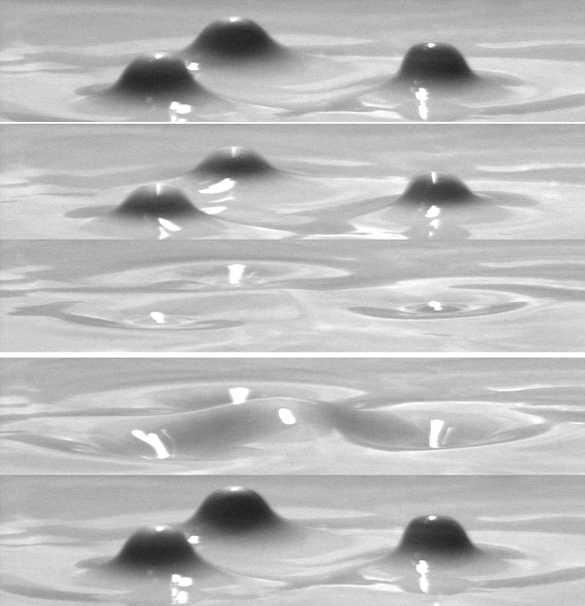
\includegraphics[width=0.5\textwidth]{plot/oscillon-non-newton.jpg}
  \caption{Granular oscillons in clay suspensions \cite{PhysRevLett.83.3190}. Image: Dr.~Oleg Lioubashevski, The Racah Institute of Physics, The Hebrew University of Jerusalem \cite{blazelab}. Three (1+2)-D oscillons are shown in this image. As can be seen here, the two-dimensional surface oscillates around the hyper-plane $u=0$, which is the horizontal plane of zero field value.}
  \label{nntliquid}
\end{figure}

Oscillons are studied in applied mathematics (Section \ref{litrev:appm}), cosmology (Section \ref{litrev:cosmo}), condensed matter physics, and non-linear optics (Section \ref{litrev:phymisc}). This Introduction will serve as a review of the vast corpus of relevant literature from different branches of mathematics and physics, to provide a unified overview of the subject.

Before we begin we will clarify terminology. In applied mathematics, the term ``breather'' is synonymous with ``oscillon'' in the sense it is used here. We will later use the phrase ``breathing behaviour'' to describe pulsating profiles in two-scale oscillons in subsequent chapters of this Thesis, but will not the use the term ``breather''.

\section{Oscillons in the Applied Mathematics}\label{litrev:appm}
In applied mathematics, certain wave equations can be understood as infinite-dimensional Hamiltonian systems \cite{intsys}, and therefore can be ``integrated'' completely using methods such as the inverse scattering transform \cite{intsys, spiro, ablowitz}. Though a universally acceptable definition of integrability does not exist for general partial differential equations \cite{intsys}, we can nevertheless characterize a wave equation by whether one can find all its solutions using some analytical procedure. This class of partial differential equations contains the standard constant-coefficient linear wave equation, which can be solved using standard separation of variable technique or the Fourier transform, and the sine-Gordon equation in 1D:
\begin{equation}
  \partial^2_t u - \partial^2_x u + \sin u = 0
\end{equation}
with the 1D sine-Gordon potential $V(u) = 1-\cos u$, which can be solved using the inverse scattering transform or the B\"acklund transformation (see Section \ref{litrev:gensolsg1d}). Other non-linear potentials (including sine-Gordon in two or more spatial dimensions) are not integrable.

It can be shown that the linear wave equation does not support meta-stable oscillon solutions \cite{Copeland:1995fq}. This section will first review oscillon solutions to the integrable 1D sine-Gordon equation and then will then look at oscillons in the more general non-integrable case.

\subsection{General Solutions to the 1D Sine-Gordon Equation}\label{litrev:gensolsg1d}

The sine-Gordon equation was first introduced in the 19th century by Edmond Bour, as the Gauss-Codazzi equation for surfaces of constant Gaussian curvature $K=-1$ in 3-space \cite{bour}. For a surface given by the graph of a $C^\infty$ function
\begin{equation}
  x^3 = f(x^1, x^2)\,,
\end{equation}
where $(x^1,x^2)\in U$ for some open set $U\subset \mathbb{R}^2$, the following Codazzi-Mainardi equation describes the so-called compatibility condition which encodes the fact that the higher order differentials of $f$ are independent of the order of differentiation\footnote{This is \emph{not} related to integrability, as far as we are aware of.}:
\begin{equation}\label{codazzi}
  h_{ij,k} - h_{ik,j} - h_{lj}\Gamma ^l{}_{ik} + h_{lk}\Gamma^l_{ij}=0\,,
\end{equation}
where $\Gamma^i{}_{jk}$ is the Christoffel symbol and $h_{ij}$ is the second fundamental form.

The sine-Gordon equation arises from applying (\ref{codazzi}) to the surface of constant Gaussian curvature $K=-1$, for which the first fundamental form \cite{do1976differential} takes
\begin{equation}
  g_{ij} = \left( \begin{array}{cc}
    1& \cos\phi\\
    \cos\phi&1
    \end{array}\right)
\end{equation}
with $\phi = \arccos \langle e_1,e_2\rangle$, where $\langle v, w\rangle$ is defined to be the inner product of vector $v$ and $w$, and the second fundamental form takes
\begin{equation}
  h_{ij} = \left( \begin{array}{cc}
    0& \sin\phi\\
    \sin\phi&0
    \end{array}\right).
\end{equation}

\begin{figure}\centering
  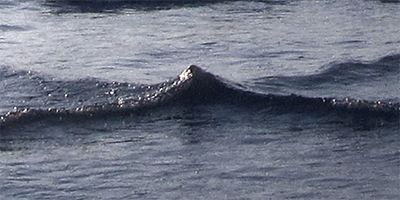
\includegraphics[width=0.7\textwidth]{plot/water-soliton.png}
  \caption{Reprint of Fig.~1(b) from \cite{PhysRevE.86.036305}, which shows a solitonic water wave.}
  \label{water}
\end{figure}

It was soon realized that the 1D sine-Gordon equation supports the so-called solitonic solutions. Solitons were originally discovered in the context of water waves (Fig.~\ref{water}), by John Scott Russell \cite{russell}, also dating back to the mid 19th century. They are termed ``solitons'' because they behave just like particles when they scatter against each other \cite{Perring:1962vs}. Solitons (at least for the exactly integrable equations) will retain their original shape without distortion after interactions, as is shown in Fig.~\ref{interaction}. Additionally, it appears that the presence of solitons is universal in a variety of non-linear wave equations, including the Korteweg-de Vries equation which describes water waves \cite{ablowitz} and the sine-Gordon equation. This generated great interest in understanding the general solitonic solutions of integrable non-linear wave equations in the 1970s, and lead to the development of the inverse scattering transform as a general method of integrating certain non-linear partial differential equations \cite{SAPM:SAPM1974534249}.

The most comprehensive review of the inverse scattering transform is the book \cite{ablowitz} by Ablowitz, one of the inventors of this method. We also note a few shorter, more accessible introductions to the topics of integrable systems, solitons and inverse scattering transform in \cite{Aktosun2009, spiro, intsys}.

Based on the inverse scattering transform, it is possible to encode all general solitonic solutions to the 1D sine-Gordon solution into a ``matrix'' form. This ``matrix'' method takes an $n\times n$ matrix along with a set of ancillary $n$-dimensional vectors as input and generates a $n$-soliton. We will later (in Chapter \ref{exactsol}) use this method to construct a novel oscillon solution to the 1D sine-Gordon equation with two independent oscillation frequencies, termed ``two-scale oscillons''. For a detailed description of this method, see the original paper \cite{:/content/aip/journal/jmp/51/12/10.1063/1.3520596}. There is also a shorter talk on this subject \cite{sgtalk}.

Another method of generating solitonic solutions to the 1D sine-Gordon equation is the B\"acklund transformation \cite{Dodd499, hietarinta1997introduction, Cuenda20111047}, which is a non-linear generalization of the super-position principle of the linear wave equation. However, we note that the B\"acklund transformation can only generate \emph{solitonic} solutions, while the inverse scattering transform can generate both solitonic and radiative solutions, and combinations thereof.

\begin{figure}\centering
  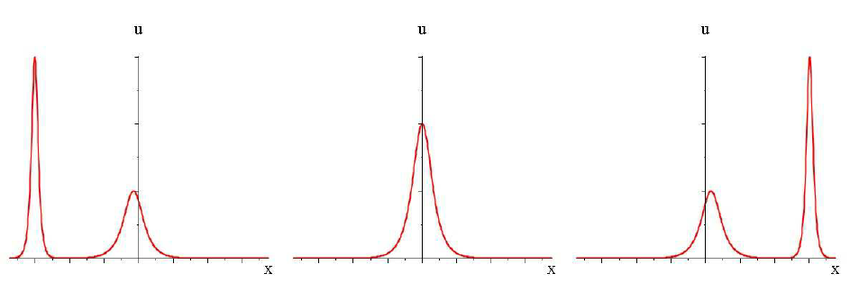
\includegraphics[width=0.9\textwidth]{plot/soliton-interaction.png}
  \caption{Reprint of Fig.~3 from \cite{2011PhyD..240.1378A}. An important property of exact solitonic solutions is that they interact and retain their original shape after interactions. This diagram shows two solitons of different shapes (left plot) interact non-linearly (middle plot) and retain their original shapes as they leave each other (right plot).}
  \label{interaction}
\end{figure}

\subsection{Generalizations of the sine-Gordon Equation}
We briefly mention some generalizations of the sine-Gordon equation that have been studied in the literature. We start with exactly integrable cases and move on to the non-integrable ones.

\subsubsection{Exactly integrable cases}
A generalization of the sine-Gordon equation is \cite{1751-8121-43-10-105204}
\begin{equation}
  u_{tx} = (1+\nu \partial^2_x)\sin u\,,
\end{equation}
where $\nu$ is a real parameter. For $\nu<0$, this equation is exactly integrable and can be shown to have novel solitonic solutions in \cite{1751-8121-43-10-105204} where the smaller solitons travels faster than the larger soliton.

\medbreak
Another  generalization of the sine-Gordon equation is the vector sine-Gordon equation:
\begin{equation}\label{vectorsg}
  \partial_t\left(\frac{\bm{\alpha}_x}{\beta}\right) = \bm{\alpha}
\end{equation}
where $\bm{\alpha}$ is a $n$-dimensional real vector field and $\beta = \sqrt{1 - \langle\bm{\alpha},\bm{\alpha}\rangle}$. We require $\langle\bm{\alpha},\bm{\alpha}\rangle\le1$ so that $\beta\in\mathbb{R}$. Taking $n=1$ and $\alpha = \sin \theta$ reduces (\ref{vectorsg}) to the standard 1D sine-Gordon equation $\theta_{tx} = \sin \theta$.

This equation is also exactly integrable. By using a Lax-pair based approach called the ``dressing method'' similar to the inverse scattering transform Ref.~\cite{Mikhailov201653} shows it is possible to obtain similar solitonic solutions to those seen in the case of 1D sine-Gordon equation.

\subsubsection{Non-integrable cases}
A different approach to generalizing the sine-Gordon equation is to add perturbation to it. For a general perturbation, this usually makes the equation non-integrable. Ref.~\cite{PhysRevB.85.134525} investigated the radiative annihilation of a soliton and an anti-soliton in the following perturbed, coupled vector sine-Gordon equation:
\begin{equation}
  \partial^2_x\phi_i=\sum_j \mathbf{A_{ij}} \left[\partial^2_t \phi_j +\alpha \phi_j +\sin \phi_j - \gamma\right],
\end{equation}
where $\alpha$ is the viscous damping parameter, $\gamma$ the driving term, and $\mathbf{A_{ij}}$ is the coupling matrix, the off-diagonal elements of which describe the interactions between different $\phi_i$ fields. This equation is not integrable, and therefore only numerical analysis was performed. It was shown in \cite{PhysRevB.85.134525} that this equation supports solitonic solutions, and soliton-anti-soliton pairs will annihilate even in the absence of perturbations, which is not the case in plain 1D sine-Gordon equations.  Ref.~\cite{RevModPhys.61.763} provided a comprehensive review of the method inverse scattering transform when applied to nearly integrable systems which are exactly integrable equations perturbed by certain treatable forms of perturbation.

\medbreak

A final generalization to the sine-Gordon equation is a slight deformation of the sine-Gordon potential. Ref.~\cite{Ferreira2011} investigated the following potential
\begin{equation}\label{deformed}
  V(\phi, n) = \frac{2}{n^2} \tan^2 \phi \left( 1 - \left|\sin\phi\right|^n \right)^2\,,
\end{equation}
which reduces to the plain sine-Gordon equation when $n=2$. The case $n=2+\epsilon$ was considered, for which $V$ can be expanded around the exact sine-Gordon potential assuming $\epsilon$ is small. This leads to the concept of ``quasi-integrability'', which allows one to obtain solitonic solutions and their asymptotic conservation laws. It was also demonstrated numerically that (\ref{deformed}) supports long-lived oscillons and other solitonic solutions.

\subsection{General Non-linear Potentials}
In general, one does not expect any form of integrability for a general non-linear wave equation. However, for certain special cases one can nonetheless construct oscillon solutions directly. An example is the swaying oscillons in the signum-Gordon model \cite{Arodz:2011zm}:
\begin{equation}
  V(\phi)=\left|\phi\right|.
\end{equation}

This type of potential supports the ``swaying'' oscillon solutions \cite{Arodz:2011zm} where the center of oscillon sways in a fixed interval periodically while the overall size of the oscillon remains strictly constant. These oscillons are exact analytic solutions.

\medbreak

For general non-linear potentials, there are two broad categories of approaches in terms of understanding the properties of oscillons: non-perturbative methods, and numerical methods. We will discuss them separately.

\subsubsection{Non-perturbative methods}\label{nonpert}
\begin{figure}\centering
  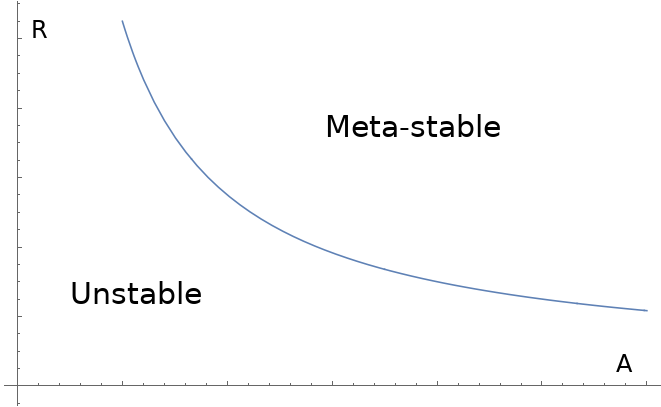
\includegraphics[width=0.5\textwidth]{plot/stability.png}
  \caption{Typical stability map starting from Gaussian initial profiles with amplitude $A$ and radius $R$.}
  \label{stability}
\end{figure}

The general non-perturbative methods for analyzing oscillon dynamics are described in detail in \cite{Copeland:1995fq, PhysRevD.80.125037, Gleiser:2008ty}. The idea is to expand the potential in power series and integrate each order in the power series separately. We will (in Chapter \ref{nonpertprob}) point out that this method has the serious limitation that it only applies to finite order polynomial potentials. It will fail on, for instance, the axion-monodromy potential \cite{McAllister:2008hb, Silverstein:2008sg, Flauger:2009ab}. Nonetheless, it is possible to establish some important properties of oscillons using this series expansion technique. The main results are:
\begin{enumerate}
\item The meta-stability of oscillons is due to the fact that the non-linear potential acting as the ``restoring force'' does not increase linearly so that outgoing radiation is greatly suppressed. In a linear theory, an initial oscillon profile will decay rapidly and no meta-stable oscillons can be formed.
\item Starting from a Gaussian initial profile $\phi(0,r)=A\exp(-r^2/R^2)$, one can obtain a stability map which typically looks like Fig.~\ref{stability}, which has a distinctive region in the parameter space where oscillons are meta-stable. Outside this region, the oscillons decay rapidly and are not stable. We will see in our numerical study of the axion-monodromy oscillons that the oscillons that live near the stable-unstable separation have strong breathing modes (see Fig.~\ref{stableunstableprofiles}.
\item Using the series expansion technique, one may establish an analytic expression for the decay rate of oscillons (eq.~(49) in \cite{PhysRevD.80.125037}). It can also be argued that there is an attractor point in the configuration space to which oscillons tend, by minimizing the effective potential obtained from the series expansion.
\end{enumerate}

\begin{figure}\centering
  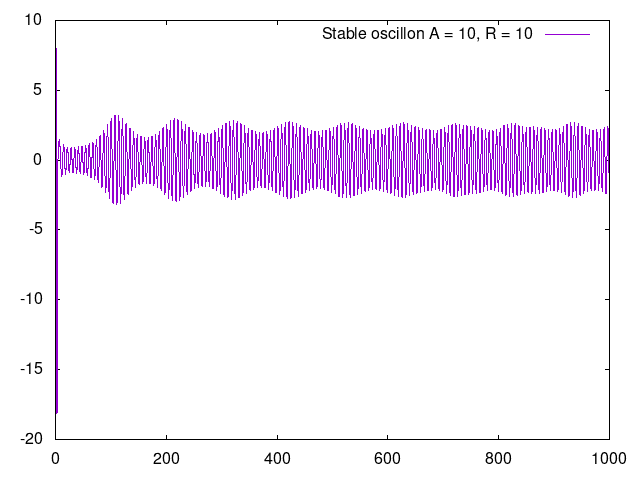
\includegraphics[width=0.6\textwidth]{plot/stable.png}\\
  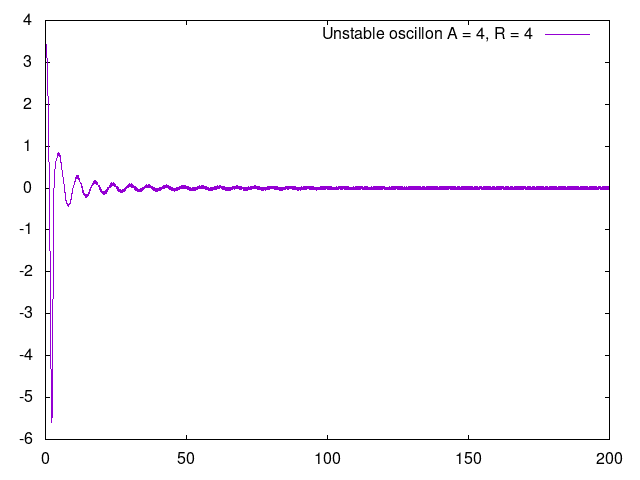
\includegraphics[width=0.6\textwidth]{plot/unstable.png}
  \caption{[TOP] Stable oscillon profile ($\phi(t,0)$) with initial Gaussian ansatz $A = 10$, $R=10$. This particular oscillon lives near the stable-unstable boundary (Fig.~\ref{stability}) and is therefore breathing.
  [BOTTOM] Unstable oscillon profile with $A = 4$, $R = 4$.}
  \label{stableunstableprofiles}
\end{figure}

Additionally, it is established in \cite{Mukaida:2016hwd} that the longevity of oscillons can be understood as the result of an effective theory with an approximate global $U(1)$ symmetry. This approximate $U(1)$ symmetry will lead to an approximate number conservation which will lend to the extreme longevity of oscillon configurations. Oscillon decay can then be understood as the breaking of this $U(1)$ symmetry via number-conservation violating processes. Both this study and the previous non-perturbative method are consistent in terms of establishing the fact that oscillon longevity is a dynamic process, where the longer time-scale appears dynamically, rather than as a parameter of the theory.

\begin{figure}
  \centering
  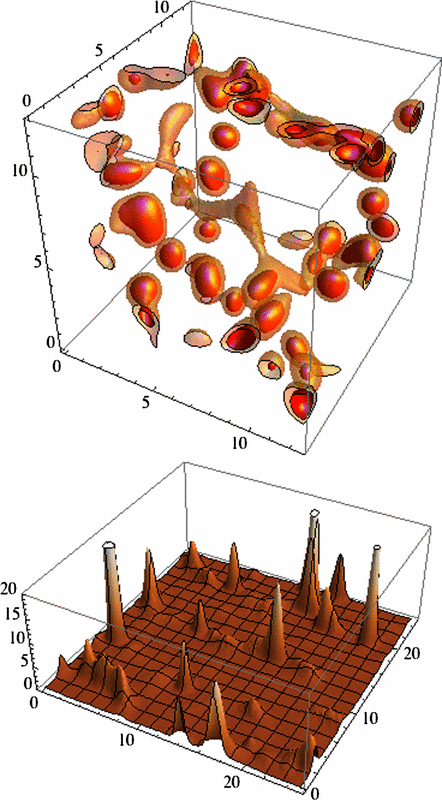
\includegraphics[width=0.6\textwidth]{plot/oscillons-2.png}
  \caption{Fig.~2 in \cite{Amin:2011hj} which shows a typical time-slice in an oscillon-dominated universe from PSpectRE \cite{Easther:2010qz} simulation. [TOP] The 3D contour plot of the simulated oscillon population at a specific time-slice. [BOTTOM] The field values of a specific spatial slice of the field configuration in the top plot.}\label{monodromyoscillons}
\end{figure}

\subsubsection{Numerical methods}
In all of the studies listed in the previous subsection, the analytical methods are accompanied with numerical studies to confirm their findings. We also note several additional numerical studies dedicated to study specific types of oscillons.

Ref.~\cite{Salmi:2012ta} studied the power spectrum of the field oscillation at the center of the oscillon, and found that at least for their specific examples, the power spectrum has a distinctive shape (see Fig.~6 of \cite{Hindmarsh:2006ur}). We will use the same methods to study the power spectrum of two-scale oscillons and find that the power spectrum has a different and distinctive shape.

Ref.~\cite{Hindmarsh:2006ur} studied oscillons in two spatial dimensions using a similar method to Ref.~\cite{Salmi:2012ta}, which mentioned their existence but did not examine them in detail. It is noteworthy that this study has found breathing modes in 2D sine-Gordon oscillons. These breathing modes are the main focus of this Thesis. We will confirm the studies done in Ref.~\cite{Hindmarsh:2006ur} and provide an analytic characterization of the breathing modes.

\section{Oscillons in the Early Universe}\label{litrev:cosmo}
Inflation is the period of cosmic evolution immediately after the Big Bang singularity where the universe underwent exponential expansion drive by an inflaton field \cite{mukhanov2005physical}. In string inflation \cite{stringInflationBook, McAllister:2008hb, Silverstein:2008sg, Flauger:2009ab}, a natural candidate for the inflaton field is the axion-monodromy potential:
\begin{equation}\label{fullampot}
  V(\phi) = \frac{m^2M^2}{2\alpha} \left[\left(1+\frac{\phi^2}{M^2}\right)^\alpha -1\right].
\end{equation}

It is established in \cite{Amin:2010dc, Amin:2011hj} that parametric resonance provides a natural and dynamical process of generating axion-monodromy oscillons in the (p)re-heating stage of the inflationary universe (see Fig.~\ref{monodromyoscillons}), where at the end of the inflation stage the self-resonance of the inflaton field will start ``pumping'' energies into the inflaton field and generate a copious amount of oscillons as a result of this self-resonance. This parametric resonance can be analyzed using Floquet theory and the existence of an oscillon dominated phase is confirmed by numerical simulation of the post-inflation universe, using PSpectRE \cite{Easther:2010qz}.

The analytic study of oscillons in an expanding universe is done in \cite{Amin:2010jq}, where it also found a new class of ``flat-top'' oscillons in the $\phi^6$ theory. The detailed Floquet analysis can be found in \cite{Amin:2010dc}.

\section{Oscillons in Other Physical Systems}\label{litrev:phymisc}
Oscillons are also observed in many condensed matter systems, including Bose-Einstein condensates \cite{umbanhowar1996localized}, nonlinear optics \cite{Copeland:2014qra}, and vibrated granular materials \cite{Tsimring:1997zz, PhysRevLett.83.3190}. In particular, \cite{PhysRevLett.83.3190} has a vivid experimental realization of the granular oscillons in shear thinning non-Newtonian liquids, shown in Fig.~\ref{nntliquid}.

We also note that in applications to nonlinear optics, the sine-Gordon equation is solved in a different boundary condition than what we are using here, namely they use periodic boundary condition for both space and time \cite{JAWORSKI1982427, 0305-4470-15-10-015}. \cite{JAWORSKI1982427, 0305-4470-15-10-015} discussed possible oscillon-like solutions in this type of boundary conditions.

\section{Note on the Numerical Methods Used in the Project}\label{intro:num}
We have two primary numerical methods in this project, a plain leap-frog integrator which solves the spherically symmetric $(1+n)$-dimensional Klein-Gordon equation, and the full numerical simulation of the axion-monodromy inflation universe, using the pseudo-spectral integrator PSpectRE \cite{Easther:2010qz}.

The plain Klein-Gordon solver is implemented as a staggered leap-frog integrator with an absorbing boundary condition, by adding an artificial numerical viscosity at large $r$. We typically start the integrator with the exact two-scale solution as the initial profile, and evolve the radial Klein-Gordon equation to obtain the full oscillon dynamics, assuming spherical symmetricity. The numerical integrator is implemented in Fortran and is available at \cite{fortrancode}.

A preliminary study \cite{josh} was done based on this numerical integrator and concluded that the axion-monodromy oscillons have a similar stability map to that shown in Fig. \ref{stability}. Furthermore, it found that as the parameters approach the transition curve between the stable and unstable regions, the axion-monodromy oscillons have strong breathing behaviours that were not previously understood analytically.
\medbreak
For the full simulation of the post-inflationary universe, we use the pseudo-spectral integrator, PSpectRE \cite{Easther:2010qz}, with modifications to allow it run on the GPUs, in order to accelerate the computations. For details, see Section \ref{porting}. The source code of the GPU version of PSpectRE can be found on \cite{cudaport}.

\section{Summary of New Results}
The main results of this Thesis are the exact analytic oscillon solution of the 1D sine-Gordon equation with two independent oscillation time scales, or the ``two-scale'' solution (Chapter \ref{exactsol} and \ref{prop}), and the extension of this exact solution to general potentials and dimensionalities, in particular, the 3D axion-monodromy potential (Chapter \ref{general}).

In Chapter \ref{appcosmo}, we derive an analytic ansatz from the exact solution and fit the oscillon profiles from the PSpectRE (Fig.~\ref{monodromyoscillons}) simulation of the axion-monodromy oscillons, and conclude that the analytic profile accounts for local, but not global, breathing behaviour of the axion-monodromy oscillons.

Finally, in Chapter \ref{nonpertprob} and Chapter \ref{chap:stability} we examine the stability of oscillons, evaluating and generalizing existing approaches based on an assumed Gaussian initial profile.

\chapter{The Series Expansion Technique}\label{nonpertprob}
\section{The Series Expansion Technique and Its Limitations}
The ``series expansion'' technique refers to the non-perturbative treatment of oscillon dynamics in a general non-linear potential, described in \cite{PhysRevD.80.125037, Gleiser:2008ty}. The idea of this method is to expand the potential $V(\phi)$ into a power series around the vacuum $\phi_0$ which we assume to be at $\phi=0$:
\begin{equation}
  V(\phi)=\sum_{n=0}^\infty \frac{g_n}{n!}\phi^n\,.
\end{equation}

Starting from the full Lagrangian
\begin{equation}\label{lagfull}
    L = \frac{2\pi^{d/2}}{\Gamma(d/2)}\int r^{d-1}\,\mathrm{d}r\left[\frac{1}{2}\dot{\phi}^2 -
      \frac{1}{2}\left(\frac{\partial\phi}{\partial r}\right)^2-V(\phi)\right],
\end{equation}
we substitute the assumed Gaussian ansatz
\begin{equation}
  \phi(r,t) = A(t) \exp\left(-\frac{r^2}{R^2}\right)
\end{equation}
into eq.~(\ref{lagfull}) and integrate out the radial part, so that the dynamics becomes that of a single variable function $A(t)$:
\begin{equation}
  L= \left(\frac{\pi}{2}\right)^{d/2}R^d\left[\frac{1}{2}\dot{A}^2 - V_{\rm eff}(A)\right].
\end{equation}

This $A(t)$ function will then have a classical motion in an effective potential $V_{\rm eff}$, where
\begin{equation}\label{effpot}
  V_{\rm eff}(A) = \frac{A^2d}{2R^2} +
  \sum_{n=0}^\infty \frac{g_n}{n!}\left(\frac{2}{n}\right)^{d/2} A^n\,.
\end{equation}

This is a valid approach for polynomial potentials (namely, potentials that are truncated power series). However, we will demonstrate here that this approach fails for more complicated potentials which have an infinite power series expansion with a finite radius of convergence. An example is the axion-monodromy potential in inflation cosmology \cite{stringInflationBook, McAllister:2008hb}:
\begin{equation}
  V(\phi) = \frac{m^2M^2}{2\alpha}\left[\left(1+\frac{\phi^2}{M^2}\right)^\alpha-1\right].
\end{equation}
We focus on $\alpha=1/2$ but our conclusions below would apply more generally.

We note that a trivial re-scaling allows us to set
\begin{equation}
  m=M=1\,.
\end{equation}
Therefore we will take
\begin{equation}\label{V}
  V(\phi)=\sqrt{1+\phi^2}-1\,.
\end{equation}

In what follows, we show that a naive application of the series expansion technique to the axion-monodromy potential does not give the right result --- the stability criterion predicts that oscillons are unstable and therefore cannot be formed, while from numerical simulations clearly show oscillon formations in both the post-inflationary universe and starting from an initial localized profile (see Section \ref{intro:num}).

To start, we expand (\ref{V}) into power series:
\begin{equation}\label{Vexpand}
  V(\phi)=\sum_{n=1}^\infty\frac{\alpha(\alpha-1)\cdots(\alpha-n+1)}{n!}\phi^{2n}\,,
\end{equation}
and note that it has a finite radius of convergence $r=1$. Substituting (\ref{Vexpand}) into (\ref{effpot}), we have
\begin{equation}\label{Veff}
  V_{\rm eff}(A)=\frac{A^2d}{2R^2} + \sum_{n=1}^\infty\frac{\alpha(\alpha-1)\cdots(\alpha-n+1)}{n!}
  \left(\frac{1}{n}\right)^{d/2}A^{2n}\,.
\end{equation}
Both sums in (\ref{V}) and (\ref{Veff}) have radius of convergence 1 and are holomorphic within their radius of convergence. In order to evaluate $V_{\rm eff}(A)$ for $A>1$, we note that the effective potential $V_{\rm eff}$ is defined as an integral in (\ref{lagfull}), and is therefore analytic in its domain. This allows us to analytically continue the second sum to obtain a meromorphic function in $\mathbb{C}$. We will denote the function thus obtained as $F(z)$. In other words,
\begin{equation}\label{VeffFz}
  V_{\rm eff}(A) = \frac{A^2d}{2R^2} + F(A)\,.
\end{equation}

To solve for $F(z)$ explicitly, note for a start that for $d=2$, differentiating $F(z)$ gives
\begin{equation}
  F'(z)=\sum_{n=1}^\infty\frac{\alpha(\alpha-1)\cdots(\alpha-n+1)}{n!} \cdot 2 z^{2n-1}\,.
\end{equation}
Therefore we have, for $d=2$,
\begin{equation}
  F'(z)=\frac{2}{z}\left[\sqrt{1+z^2}-1\right].
\end{equation}
Integrating this we have, assuming suitable branch cut,
\begin{equation}
  F(z) = 2 \left(\sqrt{z^2+1}-1-\log \frac{1+\sqrt{z^2+1}}{2}\right).
\end{equation}

We now substitute this expression for $F(z)$ into (\ref{VeffFz}), and obtain the final form of the effective potential for $d=2$:
\begin{equation}
  V_{\rm eff}(A) = \frac{A^2}{R^2} + 2 \left(\sqrt{A^2+1}-1-\log \frac{1+\sqrt{A^2+1}}{2}\right).
\end{equation}

The stability criterion in \cite{Gleiser:2008ty} states that the region where $I(A,R) = V''_{\rm eff}(A)<0$ gives meta-stable oscillon configurations. However, evaluating $V''_{\rm eff}(A)$, we have
\begin{equation}
  V''_{\rm eff}(A) = 2 \left(\frac{1}{1 + A^2 + \sqrt{1 + A^2}} + \frac{1}{R^2}\right),
\end{equation}
which is positive definite. Therefore, the stability criterion in \cite{Gleiser:2008ty} predicts no stable oscillons, which contradicts the findings of numerical simulations.

Note that this procedure is applicable for all $d$ even. Setting $d=2p$, differentiating $F(z)$ once gives
\begin{equation}
  \frac{z}{2}D_z F = \sum_{n=1}^\infty\frac{\alpha(\alpha-1)\cdots(\alpha-n+1)}{n!} \frac{1}{n^{p-1}} z^{2n}\,,
\end{equation}
where $D_z$ denotes differentiating with respect to $z$. Differentiating $F(z)$ $p$ times therefore gives
\begin{equation}
  \left(\frac{z}{2}D_z\right)^p F = V(z) = \sqrt{1+z^2}-1\,.
\end{equation}
Integrating the equation above then gives the explicit form of $F(z)$, once we take care of integration constants and branch cuts.

Another method of obtaining the same result is to evaluate the integral in (\ref{lagfull}) directly. In other words, if one substitutes the Gaussian ansatz into the full Lagrangian (\ref{lagfull}), one is faced with the evaluation of the following integral:
\begin{equation}\label{intE}
  E(\lambda) = \int^{+\infty}_0 \left[\sqrt{1+\lambda\exp(-r^2)} -1\right]r^{d-1}\,{\rm d}r
\end{equation}
where $\lambda \ge 0$.% The problem with using the series expansion method in Sicilia's paper directly for our case is that the function $\sqrt{1+\lambda z}$ has a singularity at $z=-\lambda^{-1}$, and when $\lambda$ goes above 1, the integration will hit the radius of convergence and therefore render the series expansion invalid.

For $d=2$, $E(\lambda)$ evaluates to
\begin{equation}
  \begin{split}
  E(\lambda) &= \int^{+\infty}_0 \left[\sqrt{1+\lambda \exp(-t)} -1\right]\,{\rm d}t\\
  &= -2\sqrt{1+\lambda\exp(-x)} + 2\log\left[1+\sqrt{1+\lambda\exp(-x)}\right]\Big|^{+\infty}_0\\
  &= 2\left(\sqrt{1+\lambda} -1 -\log\frac{1+\sqrt{1+\lambda}}{2}\right),
  \end{split}
\end{equation}
which is consistent with the result using analytic continuation.

\bigbreak

For odd $d$ we can numerically evaluate the integral (\ref{intE}) and again obtain the same result that $I(A,R)$ is positive definite. In evaluating $I(A,R)$ (or equivalently, $E(\lambda)$), it is useful to rewrite the $F(z)$ function in a different form, by employing the technique of fractional differentiation and integration. Defining
\begin{equation}
  (D^\alpha f)(x)= \frac{1}{\Gamma(1-\alpha)}\frac{\rm d}{{\rm d}x}\int^x_0
  \frac{f(t)}{(x-t)^\alpha}{\rm d}t
\end{equation}
and
\begin{equation}
  (J^\alpha f)(x) = \frac{1}{\Gamma(\alpha)}\int^x_0(x-t)^{\alpha-1}f(t)\,{\rm d}t
\end{equation}
as the derivative operator and the integration operator for an arbitrary (real) $\alpha$-order, respectively, it is easy to verify that they are dual to each other and that we have, for the $\frac{1}{2}$-order derivative of the basic power function $x^n$:
\begin{equation}
  D^\frac{1}{2} x^n = \frac{\Gamma(n+1)}{\Gamma(n+\frac{1}{2})} x^{n-\frac{1}{2}}\,.
\end{equation}
From this we can evaluate $D^\frac{1}{2} F$ for $d=\frac{1}{2}$:
\begin{equation}
  (D^\frac{1}{2} F)(z) = \sum^\infty_{n=1} \binom{\alpha}{n} \frac{\Gamma(2n+1)}{\Gamma(2n+\frac{1}{2})}\frac{1}{\sqrt{n}}z^{2n-\frac{1}{2}}\,.
\end{equation}
Given
\begin{equation}
  \Gamma(z)\Gamma(z+\frac{1}{2})=2^{1-2z}\sqrt{\pi}\Gamma(2z),\quad z\in\mathbb{Z}^+,
\end{equation}
we have
\begin{equation}
  \Gamma(2n+\frac{1}{2}) = \frac{2^{1-4n}}{\Gamma(2n)}\sqrt{\pi}\Gamma(4n)\,.
\end{equation}
Therefore
\begin{equation}
  (D^\frac{1}{2}F)(z) = \sum^\infty_{n=1} C_n \frac{1}{\sqrt{\pi n}} z^{2n-\frac{1}{2}}\,,
\end{equation}
where
\begin{equation}
  C_n = \binom{\frac{1}{2}}{n} \frac{(2n)!(2n-1)!}{2^{1-4n} (4n-1)!} =\binom{\frac{1}{2}}{n} \frac{(2n)\cdot(2n-1)\cdots(1)\cdot2^{4n-1}}{2n\cdot(2n+1)\cdots(4n-1)}\,.
\end{equation}
We write
\begin{equation}
  \begin{split}
    &(2n)\cdot(2n+1)\cdots(4n-1)\\
    =\,&(2n)\cdot(2n+2)\cdots(4n-2) \cdot (2n+1)\cdots(4n-1) \\
    =\,& 2^{2n}\cdot \frac{(2n-1)!}{(n-1)!}\cdot\left(n+\frac{1}{2}\right)\cdots\left(2n-\frac{1}{2}\right).
  \end{split}
\end{equation}
Therefore
\begin{equation}
  \begin{split}
    C_n &= \binom{\frac{1}{2}}{n}\frac{2n\cdot 2^{2n-1} \cdot(n-1)!}{\left(n+\frac{1}{2}\right)\cdots\left(2n-\frac{1}{2}\right)} = \binom{\frac{1}{2}}{n}\frac{2^{2n}\cdot n!}{\left(n+\frac{1}{2}\right)\cdots\left(2n-\frac{1}{2}\right)}\\
    &=\frac{\binom{\frac{1}{2}}{n}}{\binom{n-\frac{1}{2}}{n}}\cdot2^{2n} = 2^{2n}\,.
  \end{split}
\end{equation}
Plugging this back to our formula for $D^\frac{1}{2}F$, we have
\begin{equation}
  (D^\frac{1}{2}F)(z) = \frac{1}{\sqrt{\pi z}} \sum^\infty_{n=1} \frac{(4z^2)^n}{\sqrt{n}} = \frac{1}{\sqrt{\pi z}}\Li_{\frac{1}{2}}(4z^2)\,,
\end{equation}
where the polylogarithm function $\Li_s$ is defined as
\begin{equation}
  \Li_s(z) = \sum^\infty_{n=1}\frac{z^n}{n^s}\,.
\end{equation}
Therefore
\begin{equation}
  F(z) = J^\frac{1}{2}\left[\frac{1}{\sqrt{\pi z}}\Li_{\frac{1}{2}}(4z^2)\right].
\end{equation}
For positive real $z$, we have
\begin{equation}
  F(x) = \frac{1}{\pi}\int^x_0\frac{\Li_{\frac{1}{2}}(4t^2)}{\sqrt{t(x-t)}}\,{\rm d}t\,.
\end{equation}

\bigbreak

In summary, we have shown that for both $d=1$ and $d=2$, $I(A,R) = V''_{\rm eff}(A) > 0$, so the condition that $I<0$ is not satisfied for any combinations of $A$ and $R$. If we do truncate the series, as is done in Ref.~\cite{Gleiser:2008ty}, we will be able to obtain a non-trivial region where $I(A,R)<0$. However, this is not possible with the axion-monodromy potential, because the series expansion does not converge outside the radius of convergence $A = 1$ and typical oscillons have a larger amplitude than $A=1$.

\medbreak
Additionally, a further, though artificial, limitation of the series expansion technique as it is used in Ref.~\cite{Gleiser:2008ty} is that it assumes a Gaussian ansatz. We have noted in Section \ref{nonpert} that along the boarder between the stable and the unstable region, there is a proliferation of oscillons with breathing amplitudes, and therefore we would expect that the actual stable region be larger than the region given by the theoretical Gaussian model. This is not an inherent limitation, but an artificial one imposed by the choice of a Gaussian ansatz. In Chapter \ref{chap:stability} we will remedy this limitation by applying the series expansion technique to an ansatz obtained from the two-scale solution. We will show that the extended model with breathing modes enlarges the stable region and correct accounts for the numerical stability map.

\section{Attempt at Extending the Series Expansion Method}
We record here an unsuccessful attempt at extending the series expansion method. The idea is to extend the Gaussian ansatz to one with a small time dependence in the width parameter $R$, as follows:
\begin{equation}\label{wrongansatz}
  \phi(t,r) = A(t) \exp \left(-\frac{r^2}{R^2(t)}\right )
\end{equation}
where $R(t) = R_0 + \epsilon(t)$.

Substitute this into the Lagrangian, and integrate with respect to $r$ (although now $R(t)$ is time-dependent, we can still evaluate the $r$-integral at a fixed time), we have
\begin{equation}
 L = \left(\frac{\pi}{2}\right)^{d/2}\int {\rm d}t\, R^d(t) \left[ \frac{1}{2}\dot{A}^2 - V_{\rm eff} (A) +
    \mathcal{L}_1\right],
\end{equation}
where
\begin{equation}
  \mathcal{L}_1 = d\left( \dot{A}(t)A(t)\frac{\dot{R}(t)}{R(t)} +\left(1+\frac{d}{2}\right)\frac{A^2(t)}{2}\frac{\dot{R}^2(t)}{R^2(t)}\right)
\end{equation}
is the new Lagrangian density introduced by the time dependence of $R(t)$.

Assuming $\epsilon(t)$ is small at all time, the zeroth-order equation is exactly the unperturbed equation solved in the previous papers. The equation for $\epsilon(t)$, to first-order, is then a linear (ordinary) differential equation which is trivially integrated.

Assuming $A(t)=A_0\cos\omega t$, from
\begin{equation}
  \frac{\rm d}{{\rm d}t}\frac{\partial \mathcal{L}}{\partial \dot{\epsilon}} =
  \frac{\partial\mathcal{L}}{\partial \epsilon}
\end{equation}
we have,
\begin{equation}
  0 = \frac{\rm d}{{\rm d}t}\left[-\omega\sin\omega t\cos\omega t + \cos^2\omega t\left(1+\frac{d}{2}
    \right)\frac{\dot{\epsilon}(t)}{R_0}\right].
\end{equation}
Therefore we have a first integral
\begin{equation}
  C_1 = -\omega\sin\omega t\cos\omega t + \cos^2\omega t\left(1+\frac{d}{2}
  \right)\frac{\dot{\epsilon}(t)}{R_0}\,,
\end{equation}
which can then be integrated to give (we have redefined $C_1$)
\begin{equation}\label{sol}
  \frac{\epsilon(t)}{R_0}\left(1+\frac{d}{2}\right)
  = C_1\tan\omega t  - \log\cos\omega t + C_2\,.
\end{equation}

Both $C_1$ and $C_2$ are free parameters. Even after setting $C_1=C_2=0$, one is still left with the $\log$ term, which blows up at odd multiples of $\pi/2$. This renders this approach invalid.

As we have stated in the previous section, the failure of this approach is not due to an inherent limitation of the series expansion technique. Rather, it simply says that the ansatz (\ref{wrongansatz}) is non-physical. What we need to do is to find the correct, physical ansatz that reproduces the desired phenomenology. It turns out that we can indeed achieve this. This is the starting point of the two-scale solution, to which we now turn.

\chapter{The Two-scale Solution}\label{exactsol}
\section{Motivation}
The motivation for this project was to understand the dynamics of oscillons seen in axion-monodromy inflation simulations, with the broader goal of exploring other aspects of oscillon dynamics. Empirical findings obtained from numerical simulations with PSpectRE, in addition to confirming their long-livedness, point to a novel feature, namely that these oscillons have a slow breathing mode on top of the fast oscillation. This second time-scale, apart from being mentioned in passing in \cite{Salmi:2012ta}, has not otherwise been noted previously, and is therefore unexplained. Consequently, our priority is to develop a suitable analytical model for studying these breathing oscillons. Given that a simple, naive extension of the series expansion method failed to deliver the desired results, we seek a new direction.

The motivating idea is that given the 1D sine-Gordon equation is completely integrable, it would be instructive to first look at oscillon solutions in 1D sine-Gordon equation. The oscillons in 1D sine-Gordon are parameterized by a single parameter, namely their frequency $\omega\in(0,1)$, and have the following expression:
\begin{equation}\label{onescale}
  \phi(t,x) = 4 \arctan\left[ \frac{\sqrt{1-\omega^2} \cos \omega t}{\omega \cosh \sqrt{1-\omega^2} x} \right].
\end{equation}
This oscillon solution has a fixed oscillation amplitude --- in other words, it does not have any breathing modes. To add breathing modes into the oscillon solution, recall that in a linear theory, adding two sine waves with very close frequencies together will give a slow mode superimposed on top of a fast mode:
\begin{equation}
  \cos \omega t  + \cos(\omega+ \Delta\omega)t\approx \cos (\Delta\omega t/2) \cos\omega t\,.
\end{equation}
If one was able to find a analogous ``non-linear superposition'' in the 1D sine-Gordon theory, then it would be conceivable that one could construct a similar ``two-scale'' oscillon solution, namely one with two independent time scales,
\begin{equation}
  \phi(t,x) = 4\arctan (\cdots \omega_1 \cdots + \cdots \omega_2 \cdots)\,.
\end{equation}
One can then take the limit where both $\omega_i$ are close to each other will give the desired breathing mode seen in the numerical axion-monodromy oscillons.

This idea turned out to be valid. In what follows we will derive the exact two-scale solution for the 1D sine-Gordon equation, and extend it to other non-integrable potentials by numerically establishing the existence of qualitatively similar oscillons solutions in general potentials and dimensionalities.

\section{The Two-scale Solution}
The analytic form of the two-scale solution is:
\begin{equation}\label{twoscale}
  u(t,x)=4 \arctan \frac{\textrm{num}}{\textrm{denom}}\,,
\end{equation}
where the numerator mixes the space and time variables
\begin{equation}\label{num}
  \textrm{num} = \frac{\omega_1^2-\omega_2^2}{\omega_1 \omega_2} \left(\frac{\omega_1}{r_1} \cosh r_1 x \cos\omega_2 t + \frac{\omega_2}{r_2} \cosh r_2 x \cos\omega_1 t \right),
\end{equation}
where
\begin{subequations}
  \begin{align}
  r_1=\sqrt{1-\omega_1^2}\,,\\
  r_2=\sqrt{1-\omega_2^2}\,,
  \end{align}
\end{subequations}
and the denominator consists of a time-only term and a space-only term:
\begin{equation}
    \textrm{denom} = f(t) + g(x)\,,
\end{equation}
where
\begin{equation}\label{denomf}
  f(t) = \frac{\omega_1^2+\omega_2^2}{\omega_1 \omega_2} \cos \omega_1 t \cos \omega_2 t +2 \sin \omega_1 t \sin \omega_2 t\,,
\end{equation}
and
\begin{equation}\label{denomg}
  g(x) = \frac{r_1^2+r_2^2}{r_1 r_2} \cosh r_1 x \cosh r_2 x-2  \sinh r_1 x \sinh r_2 x\,.
\end{equation}

One can, of course, directly verify that this is indeed a solution to the standard sine-Gordon equation $u_{tt}-u_{xx}+\sin u=0$ by substituting the solution into the equation.

\section{Deriving the Two-scale Solution}
We now derive the two-scale solution. We will derive the result in two completely independent ways, first by using the inverse scattering transform, and next by using the B\"acklund transformations.

\subsection{The Inverse-scattering Transform Method}
The method of inverse-scattering transform is based on \cite{:/content/aip/journal/jmp/51/12/10.1063/1.3520596} which provided a compact, matrix encoding of all the solitonic solutions to the 1D sine-Gordon equation. The matrix encoding itself is derived using the inverse-scattering transform by assuming that the scattering data contains only solitonic degrees of freedom and not radiative degrees of freedom. In short, the matrix encoding takes an $n\times n$ matrix $A$, and two $n$-dimensional column vectors $B$ and $C$, to produce a $n$-soliton solution. The particular two-scale solution that we have derived uses the following input data:

\begin{equation}
A=\left(
\begin{array}{cccc}
 a_1 & b_1 & 0 & 0 \\
 -b_1 & a_1 & 0 & 0 \\
 0 & 0 & a_2 & b_2 \\
 0 & 0 & -b_2 & a_2 \\
\end{array}
\right),
\qquad B=\left(\begin{array}{c}
 0 \\
 1 \\
 0 \\
 1 \\
\end{array}\right),
\quad C=\left(\begin{array}{c}
 d_1 \\
 c_1 \\
 d_2 \\
 c_2 \\
\end{array}\right),
\end{equation}
with
\begin{subequations}\label{ivtparams}
  \begin{align}
    a_1 &=\frac{\sqrt{1-\omega_1^2}}{2}\,,\\
    a_2 &=\frac{\sqrt{1-\omega_2^2}}{2}\,,\\
    b_1 &=\frac{\omega_1}{2}\,,\\
    b_2 &=\frac{\omega_2}{2}\,,\\
    c_1 &= 2\frac{1-\omega_1^2}{\omega_1}
    \frac{\sqrt{1-\omega_1^2}+\sqrt{1-\omega_2^2}}{\sqrt{1-\omega_1^2}-\sqrt{1-\omega_2^2}}\,,\\
    c_2 &= c_1 \frac{\omega_1(1-\omega_2^2)}{\omega_2(1-\omega_1^2)}\,,\\
    d_1 &=-\frac{b_1 c_1}{a_1}\,,\\
    d_2 &=-\frac{b_2 c_2}{a_2}\,,
  \end{align}
\end{subequations}

The desired $4$-soliton solution is then obtained via
\begin{equation}
  \phi(t,x) = 4\arctan \left(\ii\,\frac{\det(I + \ii M(t,x))-\det(I - \ii M(t,x))}{\det(I + \ii M(t,x))+\det(I - \ii M(t,x))}\right),
\end{equation}
where $I$ is the identity matrix, and $M(t,x)$ is given by
\begin{equation}
  M(t,x) = \exp\left(-\frac{\beta}{2}\right)\cdot P \cdot \exp\left(-\frac{\beta}{2}\right),
\end{equation}
where $\beta(t,x) = 2Ax+A^{-1}t/2$, and $P$ is the (unique) matrix solution to the following equation:
\begin{equation}\label{lyapnov}
  AP + PA = B C^{\rm T}\,.
\end{equation}
Note that the column vector $C$ is transposed in order to produce an $n\times n$ matrix.

\medbreak

The set of parameters (\ref{ivtparams}) is obtained from a generalization of the parameter set for the 1-scale oscillon (Example 9.2 in \cite{:/content/aip/journal/jmp/51/12/10.1063/1.3520596}):
\begin{equation}
  A = \left(\begin{array}{cc}
    \omega & \sqrt{1-\omega^2}\\
    -\sqrt{1-\omega^2}&\omega
  \end{array}\right),
  \qquad B = \left(\begin{array}{c}
    0\\
    1
  \end{array}\right),
  \qquad C = \left(\begin{array}{c}
    c_2\\
    c_1
  \end{array}\right),
\end{equation}
where $c_2\neq0$. The $c_1$ and $c_2$ parameters control the phase and center of the oscillon. We would like to have the oscillon solution centered at $x=0$ and have phase shift $\phi=0$ (compared to the cosine function). We therefore require that
\begin{equation}
  c_1 \sqrt{1-\omega^2} + c_2\omega = 0\,,
\end{equation}
and
\begin{equation}
  (1-\omega^2)(c_1^2+ c_2^2) = 16\omega^2\,.
\end{equation}
These relations are obtained from the general expression for the 1-scale oscillon (Eq.~(9.2) in \cite{:/content/aip/journal/jmp/51/12/10.1063/1.3520596})
\begin{equation}
  u(x,t) = 4\arctan\frac{\rm num}{\rm denom}\,,
\end{equation}
with
\begin{subequations}
  \begin{align}
  {\rm num} &= 8a^2e^{a\zeta_+}[(ac_1-bc_2)\cos(b\zeta_-)-(bc_1+ac_2)\sin(b\zeta_-)]\,,\\
  {\rm denom} &= b^2 (c_1^2+c_2^2) + 16 a^2 (a^2+b^2)e^{2a\zeta_+}\,,\\
  \zeta_{\pm}&=2x\pm\frac{t}{2(a^2+b^2)},\qquad  a=\omega_1,\qquad b=\sqrt{1-\omega^2}\,,
  \end{align}
\end{subequations}
and setting the sine term on the numerator to 0 and the constant term on the denominator equal to the coefficient of the cosine term.

In order to obtain a two-scale oscillon (a 4-soliton solution), we duplicate the $A$ and $B$ matrices in the one-scale solution:
\begin{equation}
  A = \left(\begin{array}{cc}
    A_1 & 0\\
    0 & A_2
  \end{array}\right),
  \qquad B = \left(\begin{array}{c}
    B_1\\
    B_2
  \end{array}\right),
\end{equation}
where $A_i$ and $B_i$ ($i=1,2$) are block matrices from the one-scale parameters with $\omega\to\omega_i$.

To determine the $C$ matrix for the two-scale solution, we substitute the general form
\begin{equation}
  C = \left(\begin{array}{c}
    d_1\\
    c_1\\
    d_2\\
    c_2
  \end{array}\right)
\end{equation}
into eq.~(\ref{lyapnov}) and set coefficients in front of the sine terms on the numerator and the constant terms on the denominator to 0. The process is tedious and can be implemented using a computer algebra system such as Mathematica.

\subsection{B\"acklund Transformation}
An equally valid (and equally tedious) derivation of the two-scale solution is through the use of B\"acklund transformation \cite{Dodd499, hietarinta1997introduction, Cuenda20111047}. The idea is that the sine-Gordon equation has a symmetry that allows one to ``super-impose'' two 1-solitons to obtain a 2-soliton, as is encoded by the following Bianchi diagram \cite{Cuenda20111047}:
\[
\begin{tikzcd}
  & \text{kink}(a_1) \arrow{dr}{a_2} &&\\
  0\arrow{ur}{a_1}\arrow{dr}{a_2}&&\text{2-soliton\,.}&\\
 &\text{kink}(a_2)\arrow{ur}{a_1}&&
\end{tikzcd}
\]

More generally, given three solutions to the sine-Gordon equation $\phi_0$, $\phi_1$, $\phi_2$, the B\"acklund transformation constructs a fourth solution $\phi_{12}$ through the following ``non-linear superposition'':
\begin{equation}
  \tan \left(\frac{\phi_{12}-\phi_0}{4}\right) = \frac{a_2+a_1}{a_2-a_1} \tan \left(\frac{\phi_2-\phi_1}{4}\right),
\end{equation}
where $a_1$ and $a_2$ are arbitrary complex parameters. This is encoded succinctly by the following Bianchi diagram \cite{Cuenda20111047}:
\begin{equation}\label{bianchi}
\begin{tikzcd}
  & \phi_1 \arrow{dr}{a_2} &&\\
  \phi_0\arrow{ur}{a_1}\arrow{dr}{a_2}&&\phi_{12}\,.&\\
 &\phi_2\arrow{ur}{a_1}&&
\end{tikzcd}
\end{equation}

By doing a series of B\"acklund transformations one can derive the two-scale solution, through the following Bianchi diagram:
\begin{equation}\label{bianchitwo}
\begin{tikzcd}
  & \text{kink}(a_1) \arrow{dr}{a_1^*} &&\\
 0 \arrow{ur}{a_1} \arrow{dr}{a_1^*} & &\text{1-scale oscillon}_1\arrow{dr}{a_2}&\\
  & \text{kink}(a_1^*) \arrow{ur}{a_1} \arrow{dr}{a_2} && \text{3-soliton}\arrow{dr}{a_2^*}&\\
 0 \arrow{ur}{a_1^*} \arrow{dr}{a_2} &&\text{2-soliton}\arrow{ur}{a_1}\arrow{dr}{a_2^*}&&\text{2-scale oscillon\,.}\\
 &\text{kink}(a_2)\arrow{ur}{a_1^*}\arrow{dr}{a_2^*}&&\text{3-soliton}\arrow{ur}{a_1}\\
 0\arrow{ur}{a_2}\arrow{dr}{a_2^*}&&\text{1-scale oscillon}_2\arrow{ur}{a_1^*}\\
 &\text{kink}(a_2^*)\arrow{ur}{a_2}&&
\end{tikzcd}
\end{equation}
The intermediate states are as labeled in the above diagram.

The story is slightly different to the one for the inverse scattering transform. We cannot simply combine two one-scale oscillons through the following Bianchi diagram:
\[
\begin{tikzcd}
  & \text{1-scale oscillon}_1 \arrow{dr}{a_2} &&\\
  0 \arrow{ur}{a_1} \arrow{dr}{a_2} & &?\,.&\\
  &\text{1-scale oscillon}_2 \arrow{ur}{a_1}&&
\end{tikzcd}
\]
One can check that the resulting ``two-scale oscillon'' is \emph{not} a solution to the sine-Gordon equation. The reason is that the B\"acklund transformation method requires that the $\phi_1$ in (\ref{bianchi}) be related to the $\phi_0$ via \emph{one} single B\"acklund transformation, whereas in our case, the 1-scale oscillon is obtained via \emph{two} B\"acklund transformations.

Therefore, what we need to do to obtain the correct two-scale solution is to expand the first-order Bianchi diagram
\[
\begin{tikzcd}
  & \text{kink}(a_1) \arrow{dr}{a_1^*} &&\\
 0 \arrow{ur}{a_1} \arrow{dr}{a_1^*} & &\text{1-scale oscillon}_1&\\
   & \text{kink}(a_1^*) \arrow{ur}{a_1} &&
\end{tikzcd}
\]
by adding more initial states (that is, the vacuum solution $0$) to the diagram, and construct a 4-soliton state, as is done in diagram (\ref{bianchitwo}).

\medbreak
For both the inverse scattering method, and the B\"acklund transformation method, we provide Mathematica notebooks that carry out the required algebra automatically at \cite{mathematica}.

\chapter{Properties of the Two-scale Solution}\label{prop}
The two-scale solution is parameterized by two real numbers $\omega_1$ and $\omega_2$, both of which live in the interval $(0,1)$. The two parameters span a $(0,1)\times(0,1)$ parameter space. Depending on the values of the two parameters, the two-scale solution has a number of novel properties that are not present in one-scale oscillons. The most important feature, one that is relevant to our original goal of modeling the axion-monodromy oscillons, are the breathing modes that result from the ``non-linear superposition'' of two one-scale oscillons. A further novel feature is an off-center peak in the field profile.

The strength of these features depends on the region of the parameter space and we will qualify this with numerical metrics in Section \ref{numerical}. Finally, when $(\omega_1,\omega_2)$ is close to the $(0,0)$ corner of the parameter space, the two-scale solution is said to be in the large-amplitude limit and exhibits exotic behaviours which are very different from traditional oscillon patterns.

Before we discuss each novel feature in detail we note some general properties of the two-scale solution:
\begin{enumerate}
\item The parameter space is anti-symmetric. In other words, exchanging $\omega_1$ and $\omega_2$ gives an overall minus sign, and does not change the field dynamics.
\item Setting one of the $\omega_i$ to 1 recovers the 1-scale oscillon solution. In other words, if one lets $\omega_1\to1$, one has $r_1=\sqrt{1-\omega_1^2}\to0$, and hence $\cosh r_1 x\to1$ and $1/r_1 \to \infty$. Therefore (\ref{num}) is dominated by the
  \begin{equation}
    \frac{1-\omega^2_2}{\omega_2}\frac{\cos\omega_2 t}{r_1}
  \end{equation}
  term, and (\ref{denomg}) is dominated by the
  \begin{equation}
    \frac{r_2}{r_1}\cosh r_2 x
  \end{equation}
  term, while (\ref{denomf}) remains finite. Hence
  \begin{equation}\label{onescalep1}
    \phi(t,x) = 4\arctan \frac{\rm num}{\rm denom} = 4\arctan \frac{\frac{1-\omega^2_2}{\omega_2}\frac{\cos\omega_2 t}{r_1}}{\frac{r_2}{r_1}\cosh r_2 x}\,.
  \end{equation}
  Recall that $r_2=\sqrt{1-\omega_2^2}$, and (\ref{onescalep1}) becomes exactly the one-scale oscillon solution in (\ref{onescale}):
  \begin{equation}
    \phi(t,x) = 4\arctan \frac{\sqrt{1-\omega_2^2}\cos\omega_2 t}{\omega_2 \cosh \sqrt{1-\omega_2^2} x}\,.
  \end{equation}

\item When both $\omega_i$ are close to 1, the two-scale solution is said to be in the ``small-amplitude regime'', namely that the field amplitude goes to $0$ as both $\omega_i$ go to $1$. In general, the field amplitude grows as either $\omega_i$ moves away from $1$. If one of the $\omega_i$ is close to 0, the fraction inside $\arctan$ in (\ref{twoscale}) may exceed $\pm\infty$. We require that $\phi(t,x)$ remains continuous, which means that the $\arctan$ function will have a suitable branch chosen --- in other words, choose the desired $n$ in $\arctan v = 2\pi n+ \Arctan v$, where $\Arctan v$ is the principal value of the $\arctan$ function, so that $\phi(t,x)$ is continuous even when the inside of $\arctan$ goes to infinity.
\end{enumerate}

\section{Breathing Modes}
\begin{figure}\centering
  \includegraphics[width=0.8\textwidth]{plot/{profile-0.999-0.95}.pdf}\\\vskip20pt
  \includegraphics[width=0.8\textwidth]{plot/{profile-0.999-0.95-2}.pdf}
  \caption{3D profile plots for $\omega_1=0.999$ and $\omega_2=0.95$.}
  \label{profile1}
\end{figure}
For the two-scale solution, breathing modes are present in almost the entire parameter space (see Section \ref{numerical} for a quantitative statement). We will look at several representative examples.

Our first example is a solution in the small-amplitude regime with $\omega_1=0.999$ and $\omega_2=0.95$. Fig.~\ref{profile1} shows the 3D profile plot for this combination of parameters. We also show the 2D plot of the field at the center of the oscillon $\phi(t,0)$ at Fig.~\ref{profile2}.

As can be seen in both Fig.~\ref{profile1} and Fig.~\ref{profile2}, the two-scale solution in this particular region of parameters has the same field dynamics as the ordinary one-scale solution, except that the two-scale oscillon has a modulated width that ``breathes'' in and out in field space. In the $\phi(t,0)$ plot, this shows as the modulation of the fundamental oscillation by a slow oscillation mode.

The breathing modes can have different ``strengths'': some breathing modes are slower, while some are faster. Some are more prominent, while some are shallower. In Section~\ref{numerical}, we will give a quantitative measure for this slow mode strength. One may get a qualitative understanding by comparing the two oscillons in Fig.~\ref{profile1},~\ref{profile2} and Fig.~\ref{profile3},~\ref{profile4}.

\begin{figure}\centering
  \includegraphics[width=0.8\textwidth]{plot/{profile-0.999-0.95-3}.pdf}
  \caption{$\phi(t,0)$ plot for $\omega_1=0.999$ and $\omega_2=0.95$.}
  \label{profile2}
\end{figure}

\begin{figure}\centering
  \includegraphics[width=0.8\textwidth]{plot/{profile-0.9-0.95}.pdf}\\\vskip20pt
  \includegraphics[width=0.8\textwidth]{plot/{profile-0.9-0.95-2}.pdf}
  \caption{3D profile plots for $\omega_1=0.9$ and $\omega_2=0.95$.}
  \label{profile3}
\end{figure}

\begin{figure}\centering
  \includegraphics[width=0.8\textwidth]{plot/{profile-0.9-0.95-3}.pdf}
  \caption{$\phi(t,0)$ plot for $\omega_1=0.9$ and $\omega_2=0.95$.}
  \label{profile4}
\end{figure}

\section{Off-center Peaks}
Another prominent feature of the two-scale solution is the off-center peaks in the field profile, which is present in the second example in the previous section, with $\omega_1=0.9$ and $\omega_2=0.95$ (Fig.~\ref{profile3} and Fig.~\ref{profile4}). We can get a better understanding of the typical profile with an off-center peak by plotting the field profile at $t=0$. We plot $\phi(0,x)$ for $\omega_1=0.9$ and $\omega_2=0.95$ in Fig.~\ref{dpeak1}.

\begin{figure}\centering
  \includegraphics[width=0.8\textwidth]{plot/{profile-0.9-0.95-4}.pdf}
  \caption{$\phi(0,x)$ plot for $\omega_1=0.9$ and $\omega_2=0.95$.}
  \label{dpeak1}
\end{figure}

As can be seen in Fig.~\ref{dpeak1}, the field profile has symmetric off-center peaks, rather than one centered peak as is the case for ordinary one-scale oscillons. These two peaks will move to and from each other in the course of the oscillon lifetime, as a result of the non-linear interaction of the sine-Gordon potential. In order to present this in a more friendly way, we have provided online animations for this and other two-scale oscillons at \cite{website}.

The displacement of the peak depends on $(\omega_1,\omega_2)$ and is quantified in Section \ref{numerical}.

We can also derive an analytic form for the peak displacement at $t=0$, in the limit where $\delta=\omega_1-\omega_2$ is small, by finding the $x$ values for which the denominator in (\ref{twoscale}) is minimized:
\begin{equation}\label{disp}
  x_d = \frac{1}{2\mu}\cosh^{-1}\left(\frac{2\mu^4}{3\omega^4}\left(1-\frac{2\omega}{\delta}
  +\frac{4\omega^2}{\delta^2}\right)-1\right),
\end{equation}
where $\omega=\omega_1$ and $\mu=\sqrt{1-\omega^2}$. In other words, the closer the two frequencies, the more prominent the double peaks are. In Section \ref{numerical} we will present a numerical test for the average double peak displacement across the oscillon life-time. We will see that the numerical result is consistent with the analysis here.

To give another example of the double peak structure, we have plotted the various time-slices in the oscillon evolution for $\omega_1=0.4$ and $\omega_2=0.7$ in Fig.~\ref{dpeak2}.


\newgeometry{margin=1cm,footskip=0pt}
\begin{figure}
  \centering
  \includegraphics[width=0.4\textwidth]{plot/{profile-0.4-0.7-1}.pdf}\qquad
  \includegraphics[width=0.4\textwidth]{plot/{profile-0.4-0.7-2}.pdf}\\
  \includegraphics[width=0.4\textwidth]{plot/{profile-0.4-0.7-3}.pdf}\qquad
  \includegraphics[width=0.4\textwidth]{plot/{profile-0.4-0.7-4}.pdf}
  \caption{Various time-slices for $\omega_1=0.4$ and $\omega_2=0.7$.}
  \label{dpeak2}
\end{figure}

\begin{figure}
  \centering
  \includegraphics[width=0.4\textwidth]{plot/{profile-0.01-0.99-1}.pdf}\qquad
  \includegraphics[width=0.4\textwidth]{plot/{profile-0.01-0.99-2}.pdf}\\
  \includegraphics[width=0.4\textwidth]{plot/{profile-0.01-0.99-3}.pdf}\qquad
  \includegraphics[width=0.4\textwidth]{plot/{profile-0.01-0.99-4}.pdf}
  \caption{Various time-slices for $\omega_1=0.01$ and $\omega_2=0.99$ (Part 1). See Fig.~\ref{largeamp1cont} for Part 2.}
  \label{largeamp1}
\end{figure}

\begin{figure}
  \centering
  \includegraphics[width=0.4\textwidth]{plot/{profile-0.01-0.99-5}.pdf}\qquad
  \includegraphics[width=0.4\textwidth]{plot/{profile-0.01-0.99-6}.pdf}\\
  \includegraphics[width=0.4\textwidth]{plot/{profile-0.01-0.99-7}.pdf}\qquad
  \includegraphics[width=0.4\textwidth]{plot/{profile-0.01-0.99-8}.pdf}
  \caption{$\omega_1=0.01$ and $\omega_2=0.99$ continued. Note that the oscillon profiles have flipped over compared to Fig.~\ref{largeamp1}.}
  \label{largeamp1cont}
\end{figure}

\begin{figure}\centering
  \includegraphics[width=0.4\textwidth]{plot/{profile-0.01-0.5-1}.pdf}\qquad
  \includegraphics[width=0.4\textwidth]{plot/{profile-0.01-0.5-2}.pdf}\\
  \includegraphics[width=0.4\textwidth]{plot/{profile-0.01-0.5-3}.pdf}\qquad
  \includegraphics[width=0.4\textwidth]{plot/{profile-0.01-0.5-4}.pdf}
  \caption{Various time-slices for $\omega_1=0.01$ and $\omega_2=0.5$. As is in the previous case, the profile will flip over at around $t=200$.}
  \label{largeamp2}
\end{figure}

\restoregeometry

\section{Large-amplitude Limit}
In the large-amplitude limit, where one of $\omega_i$ is very close to 0, we can see exotic field profile dynamics that is very different from ordinary oscillon dynamics. We will illustrate this point by looking at some specific examples.

An example is $\omega_1=0.01$ and $\omega_2=0.99$, which we have plotted in Fig.~\ref{largeamp1} and Fig.~\ref{largeamp1cont}. As can be seen from the time-slice plots, the field dynamics is that of a fixed, one-scale oscillon with a small vibration mode on top of it. The field dynamics no longer has the characteristic oscillon pattern where the field profile periodically oscillates around the vacuum value $\phi=0$. The reader can view the animation of this oscillon solution at \cite{website}.

If $\omega_2$ is not close to 1 (while keeping $\omega_1$ close to 0), one can have a large-amplitude two-scale oscillon with off-center peaks that interact with each other. An example is the case with $\omega_1=0.01$ and $\omega_2=0.5$, which is shown in Fig.~\ref{largeamp2}. The field dynamics is also void of the characteristic oscillon pattern, but has a double peak which interacts non-linearly and swings around each other.

\chapter{General Potential and Dimensionality: Numerical Studies}\label{general}\chaptermark{General Potential and Dimensionality}

In this Chapter we will extend our two-scale oscillon solution for the 1D sine-Gordon equation to wave equations with a general non-linear potential and in 1, 2, and 3 spatial dimensions. We will provide three numerical metrics to assess the qualitative features that we have described in the previous chapter, and show that the general features of the exact two-scale solution, namely the breathing modes and the off-center peaks, are present in more general settings. In order to be more specific, we will study both the axion-monodromy potential
\begin{equation}
  V(\phi) = \sqrt{1+\phi^2}-1 \label{axion-potential}
\end{equation}
and the $\phi^6$ potential
\begin{equation}\label{phi6pot}
  V(\phi) = \frac{\phi^2}{2} - \frac{\phi^4}{4!} +g \frac{ \phi^6}{6!}
\end{equation}
in 1, 2, and 3 spatial dimensions, as well as the sine-Gordon potential in 2 and 3 spatial dimensions. We have scaled out the extra parameters in eq.~(\ref{fullampot}) as well as the general $\phi^6$ potential without loss of generality.

As stated in Section \ref{intro:num}, we use a staggered leap-frog integrator with an absorbing boundary condition to integrate the radial Klein-Gordon equation numerically. We start the integrator with the exact two-scale solution and evolve the radial Klein-Gordon equation to obtain the full oscillon dynamics.

\section{Numerical Metrics}\label{numerical}
We will use three numerical metrics to assess whether oscillons with two-scale features are present in more general potentials and dimensionalities.  The first is the fraction of the initial energy contained within a resulting oscillon --- if this fraction is small,  the resulting solution likely has little in common with initial state, as the majority of the energy supplied by the initial configuration has  been radiated away. Recall that the energy density is:
\begin{equation}
  e(t,r) = \frac{1}{2}\left(\left(\partial_t\phi\right)^2+ \nabla \phi\cdot \nabla \phi \right) + V(\phi) \, .
\end{equation}
The numerical integrator will integrate the energy density within a given box $r_0$ and can output ratio of final energy to initial energy within the simulation box, denoted by $E/E_{\rm init}$. Note that in cases where oscillons do not form, the energy in the initial configuration is converted to outgoing spherical waves.

The second qualitative criterion assesses the existence and stability of the off-centered peaks. For this purpose we will use
\begin{equation}
  \langle r_{\rm max} \rangle  = \left\langle \argmax_{r < r_0} |\phi(t,r)| \right\rangle_t
\end{equation}
which is the time average of the peak radius. A non-zero value indicates an off-centered peak that exists for a sufficiently long time. We will ignore outgoing radiation by only considering the field values within a suitably chosen radius $r_0$.

The third numerical metric indicates the ``strength'' of the breathing behaviours we described earlier. To this end, we will look at the field values at the origin which, if the oscillon is breathing, will have a slow mode superimposed on the fast mode. We will use the average period of the slow mode multiplied by the average amplitude to indicate the ``strength'' of the breathing behaviour. We will denote this quantity by $S$.

It is instructive to look at these three numerical metrics for the exact two-scale solution for 1D sine-Gordon. The quantity $E/E_{\rm init}$ will necessarily be 1, as the oscillons are stable and live infinitely long, and therefore do not produce any energy loss through radiation.

\begin{figure}
  \centering
  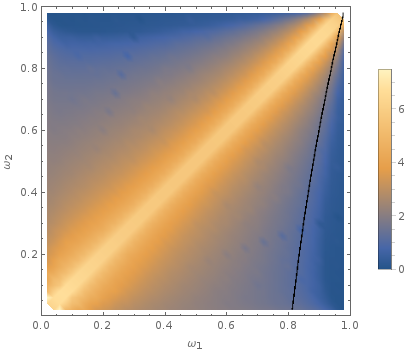
\includegraphics[width=0.6\textwidth]{plot/r_max-sine-1d.png}\\\vskip20pt
  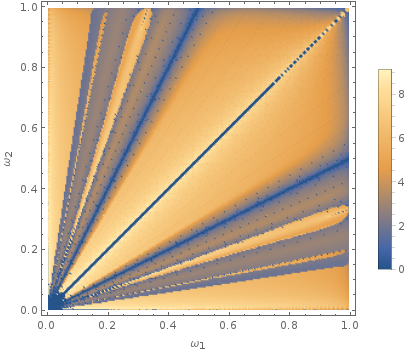
\includegraphics[width=0.6\textwidth]{plot/slow-mode-sine-1d.png}
  \caption{Values $\langle r_{\rm max}\rangle$ (upper) and  $\log{S}$ (lower) for 1D sine-Gordon. The black line is the boundary of the region with imaginary $x_d$ in eq.~(\ref{disp}).}\label{sine-1d}
\end{figure}

Next we look at the values of $\langle r_{\rm max}\rangle$ and $\log{S}$ for 1D sine-Gordon, which are plotted in Fig.~\ref{sine-1d}. The plot of $\langle r_{\rm max}\rangle$ indicates that there is a region in the parameter space, near $\omega_1=1$, where the peak displacement disappear and the oscillons are singly peaked. This is consistent with our analytical result in (\ref{disp}): if one plots the line (see Fig.~\ref{sine-1d}) where the inside of the $\cosh^{-1}$ crosses 1, thus rendering $x_d$ imaginary, one obtains the same boundary of the blue-coloured region in the $\langle r_{\rm max}\rangle$ plot with $r_{\rm max}=0$.

The $\log S$ plot for 1D sine-Gordon indicates that near the diagonal line, as well as the lower triangle in the parameter space, there are stronger breathing modes than other regions. The fact that the region near the diagonal line has strong breathing modes is explained by the interference of two single-scale oscillon, as is the case in the linear theory. The triangular region near the bottom has large $\log S$ because of the exotic behaviours in the large-amplitude limit.

\newgeometry{margin=1cm,footskip=0pt}
\begin{figure}[p]
    \centering
    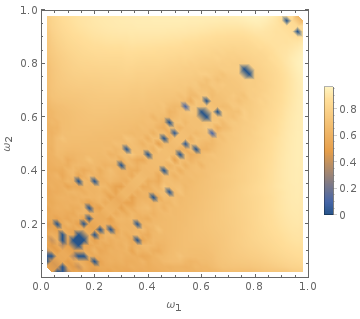
\includegraphics[width=0.3\textwidth]{plot/energy-ratio-axion-1d.png}
    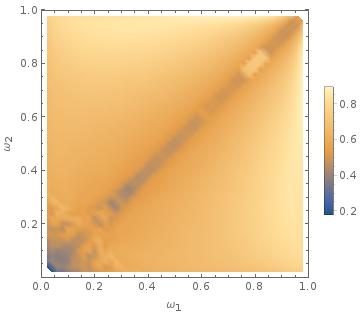
\includegraphics[width=0.3\textwidth]{plot/energy-ratio-axion-2d.png}
    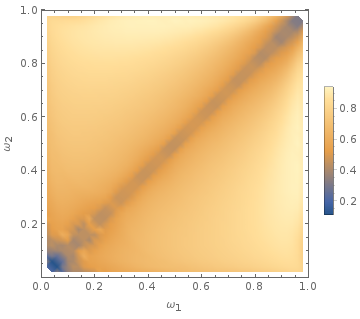
\includegraphics[width=0.3\textwidth]{plot/energy-ratio-axion-3d.png} \\
    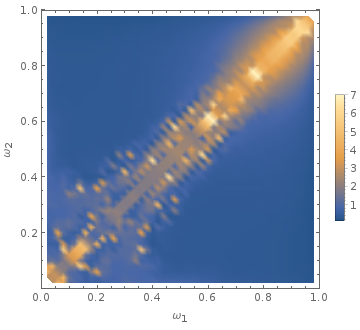
\includegraphics[width=0.3\textwidth]{plot/r_max-axion-1d.png}
    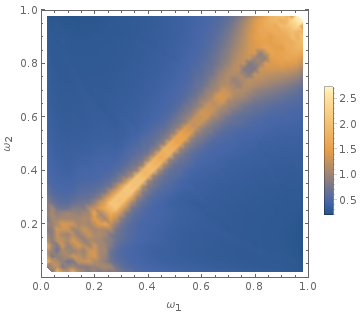
\includegraphics[width=0.3\textwidth]{plot/r_max-axion-2d.png}
    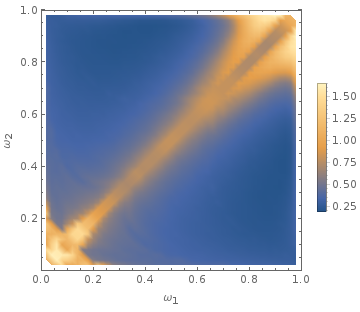
\includegraphics[width=0.3\textwidth]{plot/r_max-axion-3d.png} \\
    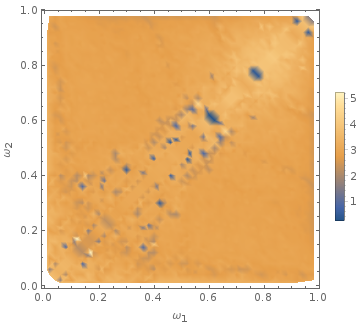
\includegraphics[width=0.3\textwidth]{plot/slow-mode-logscale-axion-1d.png}
    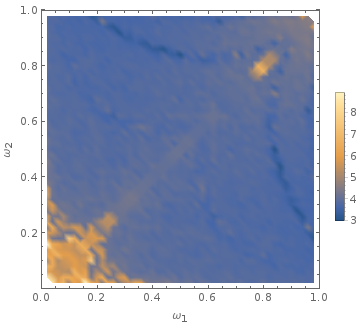
\includegraphics[width=0.3\textwidth]{plot/slow-mode-logscale-axion-2d.png}
    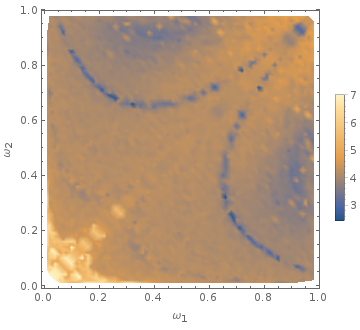
\includegraphics[width=0.3\textwidth]{plot/slow-mode-logscale-axion-3d.png}
    \caption{Qualitative properties of pulsating oscillon solutions for the axion monodromy potential. Top row: $E/E_{\rm init}$ at $t=4000$.
      Middle row: $\langle r_{\rm max}\rangle$.
      Bottom row: Strength of slow modes, $\log{S}$.\quad
      Left to right: 1D, 2D, 3D. We see that 50\% of the initial energy typically remains in the oscillon, and the peak is displaced furthest from the origin when $\omega_1 \approx \omega_2$. All choices of  $\omega_1$ and $\omega_2$ lead to a pulsating envelope, which is most pronounced when $\omega_1$ and $\omega_2$ are small in 2D and 3D. The ``holes'' in the 1D solution are associated with cases where the initial profile splits into two single oscillons moving away from the origin.}\label{axion-monodromy}
\end{figure}
\restoregeometry

\section{Axion-monodromy Potential}
We computed the three numerical metrics for the axion-monodromy potential (\ref {axion-potential}) in 1, 2, and 3 spatial dimensions. We wish to study this potential as it is a candidate for the inflaton field and provides a physical example where the post-inflationary universe may be dominated by oscillons (see Section \ref{litrev:cosmo} and Chapter \ref{appcosmo}). 

As can be seen in Fig.~\ref{axion-monodromy}, in almost all regions of the parameter space, we see that the axion-monodromy oscillons initialized with the exact two-scale solution retain $>50\%$ of their initial energies. This means that the axion-monodromy two-scale oscillons share a reasonable similarity with the two-scale 1D sine-Gordon oscillons in terms of their field dynamics, given that a significant portion of the initial energy stays within the oscillon and does not radiate away when settling into the stable oscillon configuration. This enables us to model the axion-monodromy oscillons that we have obtained in the early universe simulation with the ansatz provided by the exact 1D sine-Gordon solution, a challenge we will take up in Chapter \ref{appcosmo}.

For $\langle r_{\rm max}\rangle$ and $\log S$, we see a similar dependence on $(\omega_1,\omega_2)$ parameters to the 1D sine-Gordon case: significant pulsations were observed in the most of the $(\omega_1,\omega_2)$ space.
 
\section{Sine-Gordon Potential in 2 and 3D}

We plot the three qualitative measures for the sine-Gordon potential in 2D and 3D in Fig.~\ref{sine2d3d}. From the $\langle r_{\rm max}\rangle$ and $\log{S}$, as well as from examining the field evolution directly, we find that there exist long-lived, pulsating oscillons in 2D sine-Gordon (in agreement with  \cite{Hindmarsh:2006ur}). However, from the energy conservation heat-map $E/E_{\rm init}$ is much less than unity, suggesting these oscillons are less closely related to their exact 1D analogues. In 3D, our initial ansatz does not yield stable oscillons over most of the $(\omega_1,\omega_2)$ plane.

\section{$\phi^6$ Potential}
For the $\phi^6$ potential (\ref{phi6pot}), we find that when $g$ is small, it supports pulsating oscillons in 1, 2 and 3D near the $(1,1)$ corner of the parameter space (see Fig.~\ref{phi6}). As $g$ grows, the region which supports oscillons becomes smaller and smaller. For $g\gg 1$, two-scale oscillons exist only if  $\omega_1$ and $\omega_2$ are extremely close to unity. In Fig.~\ref{phi6} we show the result for a moderate value $g=1$, where a reasonably substantial region of the parameter space supports two-scale oscillons. When $g=2$, the region with stable oscillons shrinks and only $(\omega_1,\omega_2)$ that are very close to $(1,1)$ can support stable oscillons (Fig.~\ref{phi6g2}).

\newgeometry{footskip=100pt}
\begin{figure}[p]
  \centering
  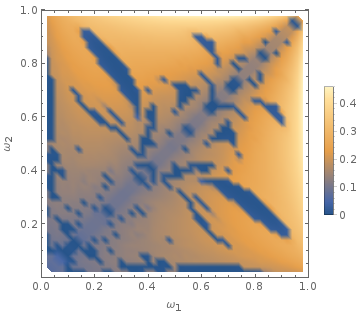
\includegraphics[width=0.45\textwidth]{plot/energy-ratio-sine-2d.png}
  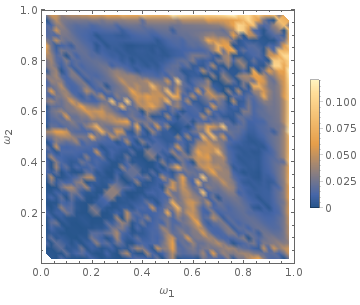
\includegraphics[width=0.45\textwidth]{plot/energy-ratio-sine-3d.png} \\
  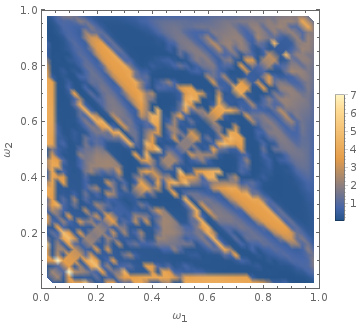
\includegraphics[width=0.45\textwidth]{plot/r_max-sine-2d.png}
  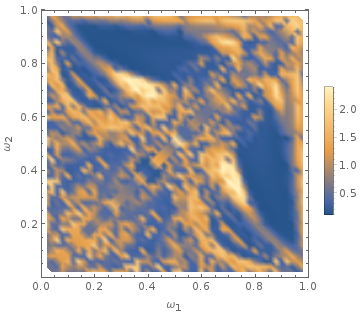
\includegraphics[width=0.45\textwidth]{plot/r_max-sine-3d.png} \\
  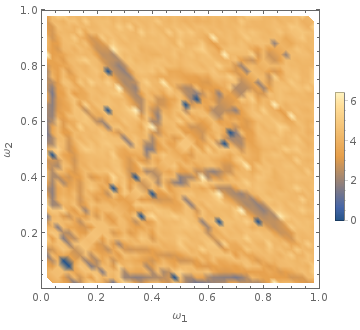
\includegraphics[width=0.45\textwidth]{plot/slow-mode-logscale-sine-2d.png}
  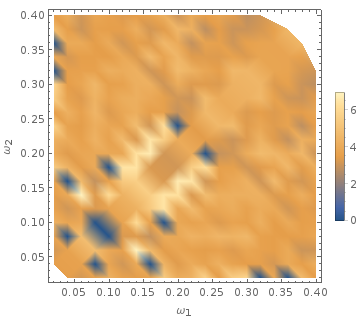
\includegraphics[width=0.45\textwidth]{plot/slow-mode-logscale-sine-3d.png}
  \caption{Qualitative properties of pulsating oscillon solutions for the sine-Gordon potential. Top row: $E/E_{\rm init}$ at $t=4000$.
    Middle row: $\langle r_{\rm max}\rangle$.
    Bottom row: Strength of slow modes, $\log{S}$.\quad
    Left to right: 2D, 3D.\qquad From the energy conservation heat-map, we find that pulsating oscillons in 2D sine-Gordon share less similarity with the exact 1D sine-Gordon solutions. For 3D sine-Gordon, the oscillons starting from the two-scale ansatz are not stable.}\label{sine2d3d}
\end{figure}
\restoregeometry

\newgeometry{margin=1cm,footskip=0pt}
\begin{figure}[p]
    \centering
    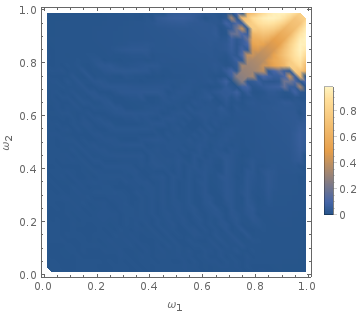
\includegraphics[width=0.3\textwidth]{plot/energy-ratio-phi6-1d.png}
    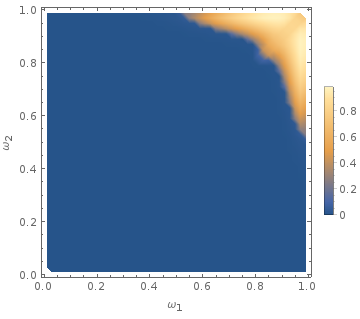
\includegraphics[width=0.3\textwidth]{plot/energy-ratio-phi6-2d.png}
    \includegraphics[width=0.3\textwidth]{plot/energy-ratio-phi6-3d.png} \\
    \includegraphics[width=0.3\textwidth]{plot/r_max-phi6-1d.png}
    \includegraphics[width=0.3\textwidth]{plot/r_max-phi6-2d.png}
    \includegraphics[width=0.3\textwidth]{plot/r_max-phi6-3d.png} \\
    \includegraphics[width=0.3\textwidth]{plot/slow-mode-logscale-phi6-1d.png}
    \includegraphics[width=0.3\textwidth]{plot/slow-mode-logscale-phi6-2d.png}
    \includegraphics[width=0.3\textwidth]{plot/slow-mode-logscale-phi6-3d.png}
    \caption{Qualitative properties of pulsating oscillon solutions for the $\phi^6$ potential with $g=1$. Top row: $E/E_{\rm init}$ at $t=4000$.
      Middle row: $\langle r_{\rm max}\rangle$.
      Bottom row: Strength of slow modes, $\log{S}$.\quad
      Left to right: 1D, 2D, 3D. \qquad What we have shown here is a moderate value of $g$, where a reasonably substantial region of the parameter space supports two-scale oscillons. If $g$ is significantly larger than $1$, the region which supports two-scale oscillons will be diminishingly small (see Fig.~\ref{phi6g2}).}\label{phi6}
\end{figure}
\restoregeometry

\begin{figure}
    \centering
    \includegraphics[width=0.45\textwidth]{plot/energy-ratio-phi6-1d-g_2.png}\\
    \includegraphics[width=0.45\textwidth]{plot/r_max-phi6-1d-g_2.png}\\
    \includegraphics[width=0.45\textwidth]{plot/slow-mode-logscale-phi6-1d-g_2.png}\\
    \caption{For $g=2$, the region with stable oscillons is significantly smaller than that of $g=1$.}\label{phi6g2}
\end{figure}

\chapter{Axion-Monodromy Inflation}\label{appcosmo}

In this Chapter, we use the results of the previous two Chapters to explore the overlap between the solutions we found in Chapter \ref{exactsol} and \ref{general} with those seen in the full simulation of the post-inflationary universe. The literature that we have reviewed in Section \ref{litrev:cosmo} suggest that in a class of string inflation models, at the end of the inflation stage the self-resonance of the inflaton field will start ``pumping'' energy into oscillons and generate an oscillon-dominated phase in the (p)re-heating stage of the universe. We will use PSpectRE \cite{Easther:2010qz} to simulate the axion-monodromy inflaton field within an expanding universe, and evolve the field dynamics to obtain an oscillon-dominated universe. We will then cut out the oscillon profiles from the simulated universe through a series of post-processing procedures on the raw simulated data. From the numerical oscillon profiles, we will use an ansatz obtained from the small-amplitude limit of the exact two-scale solution to obtain an analytic fit, and find that the analytic model gives a tolerable fit to many, but not all, of the simulated oscillons in the early universe.

\section{PSpectRE and the Simulation Settings}
PSpectRE \cite{Easther:2010qz} is a Fourier-space pseudo-spectral methods that simulates interacting scalar fields in an expanding universe. It is written in C++ and can optionally target OpenMP to utilize the multi-core capability of a modern CPU. The simulation settings, as well as the full source code that we used in this project are available in \cite{pspectregh}.

A representative time-slice of the oscillon-dominated phase in the simulated universe is shown in Fig.~\ref{oscillons}. The diagram represents the contour plot of the energy density of the axion-monodromy inflaton field. The orange blobs in the diagram are regions with individual oscillons, and are surfaces of equal energy density, and the gray contours are equal-density contours of 4 times the energy density on the surface of the oscillons.

We have plotted the field value at the center of a particular oscillon in the simulation in Fig.~\ref{raw}. As can be seen in this diagram, in general, the oscillons from our simulation have strong breathing modes with more complex dynamics than can be fully encoded with the two-scale solution. Nonetheless, we can use the two-scale solution to achieve a reasonably good fit for many of the oscillons from the simulation, accounting for most of the local breathing dynamics but not necessarily global, long-term evolution.

The oscillons from the PSpectRE simulations do not have off-center peaks, as can be seen in Fig.~\ref{oscillons}.

\begin{figure}
  \centering
  \includegraphics[width=0.6\textwidth]{plot/3dRE.png}
  \caption{Oscillons following monodromy inflation  \cite{Easther:2010qz}. Contours show regions of mean and 4 $\times$ mean density. }\label{oscillons}
\end{figure}

\begin{figure}
  \centering
  \includegraphics[width=0.7\textwidth]{plot/3Doscillon.png} 
    \caption{Central value of an oscillon extracted from full 3D numerical solution.}
  \label{raw}
\end{figure}

\subsection{Side-quest: Porting PSpectRE to CUDA}\label{porting}
The original PSpectRE code targets OpenMP for accelerating the vector operations that comprise the bulk of the computations done in the simulation. Due to their highly parallelizable nature, these vector operations are an ideal candidate for parallelizing using the GPU. A modern GPU can spawn thousands of threads in parallel, while in comparison a typical desktop CPU has only four processor cores. Therefore, porting PSpectRE to the GPU will theoretically result in a huge speed-up, if the new code respects the memory and processing model of the GPU, which has significant differences from the ordinary CPU computing model.

In running the simulations during this project, the original PSpectRE code encountered limitations from computational speed. It was therefore deemed profitable to spend some time porting PSpectRE to the GPU, in anticipation of the relatively numerous simulations that would be done. The relevant portion of the PSpectRE code has now been ported to the CUDA computing platform which targets modern NVidia Opus, and is available at \cite{cudaport}.

Note that only the features that are required in this project have been ported to CUDA. The rest of the functions have been stripped from the code-base to simplify the porting process. It is, however, a relatively trivial matter to port the rest of the features over, as they are simple vector operations that share great similarity with each other.

While it is difficult to give a rigorous performance metric, we note that for a typical simulation with $N=128$ grid points for each axis, and a total simulated time $T=1500$, the CPU version of PSpectRE takes multiple days while the GPU version runs to completion under two hours.

\section{The Small-amplitude Limit}
It is possible to derive an approximate expression for the two-scale solution, valid for the region of the parameter space that contains the numerical axion-monodromy oscillons. This approximate solution will be used as an ansatz to fit the numerical oscillon profiles in the next Section. For the full solution eqs.~(\ref{twoscale})--(\ref{denomg}), we first note that when $\omega_1\approx\omega_2$, we have
\begin{equation}
  \frac{\omega_1^2+\omega_2^2}{\omega_1 \omega_2} \approx 2\,,
\end{equation}
and likewise for $r_i$. We can therefore collect the cosine and $\cosh$ terms in the denominator eq.~(\ref{denomf}) and (\ref{denomg}) into one single term:
\begin{equation}
  f(t) \approx \cos (\omega_1-\omega_2) t\,,
\end{equation}
and
\begin{equation}
  g(x) \approx \cosh (r_1-r_2) x\,.
\end{equation}

For the numerator, we will use the trigonometric identity
\begin{equation}
  a\cos x + b \cos(x+\theta) = c \cos(x+\phi)\,,
\end{equation}
where
\begin{equation}
  c = \sqrt{a^2+b^2+2ab\cos\theta}\,,
\end{equation}
and
\begin{equation}
  \phi=\arctan \frac{b\sin\theta}{a+b\cos\theta}\,.
\end{equation}

To simplify the notation and reflect the fact that $\omega_1$ and $\omega_2$ are close to each other, we set $\omega=\omega_1$ and $\delta=\omega_1-\omega_2>0$. Note that when both $\omega_i\to1$, we necessarily have $\delta\to0$, and $r_1-r_2\approx \omega \delta/\sqrt{1-\omega^2}$.

The numerator is then proportional to
\begin{equation}
  \sqrt{2\cosh^2 rx + 2\cosh^2 (rx) \cos(\delta t)}\cos(\omega t+\phi)\,,
\end{equation}
where $\phi = -\delta t/2$ and therefore $\cos(\omega t+\phi)=\cos((\omega_1+\omega_2)t/2)\approx\cos\omega t$.

The full solution then becomes
\begin{equation}\label{approxexpr}
  u(t,x) \approx 8\sqrt{2}  \frac{\delta}{\sqrt{1-\omega^2}} \sqrt{1+\cos\delta t} \cos\omega t \frac{\cosh \sqrt{1-\omega^2} x}{\cosh(\omega\delta x/\sqrt{1-\omega^2}) + \cos \delta t}\,.
\end{equation}

For this approximate expression to apply we need $(1-\omega^2)/\omega < \delta$. Otherwise, the denominator in  (\ref{approxexpr}) goes to 0, and the expression goes to infinity.

\section{Fitting against the Two-scale Solution}

\begin{figure}
  \centering
  \includegraphics[width=0.8\textwidth]{plot/simul-profile.png}
  \caption{[Blue] Field value at the center of an oscillon from 3D monodromy simulation. [Orange] Fitted profile eq.~(\ref{fitprof}); $A=0.863$, $\omega=0.946$, $\epsilon=0.91$,  $\delta=0.046$.}\label{simul-prof}
\end{figure}

From (\ref{approxexpr}), we can generalize the approximate expression to obtain an ansatz that captures the essential, local dynamics of the numerical axion-monodromy oscillons. We will absorb the constant term $8\sqrt{2}  \delta/\sqrt{1-\omega^2}$ in front of the expression inside the $\arctan$ function into the amplitude parameter $A$, and the term $\sqrt{1-\omega^2}/\omega\delta$ inside the $\cosh$ term in the denominator into the width parameter $R$. We also note that as $\omega\to1$, the term in the numerator $\cosh\sqrt{1-\omega^2} x\to1$, and may therefore be set it to 1. The approximate solution then becomes
\begin{equation}
  u(t,x) \approx A \cos\omega t \frac{\sqrt{1+\cos\delta t} }{\cosh(x/R) + \cos \delta t}\,.
\end{equation}

In order to account for the different breathing mode amplitudes in the simulated oscillons, and to remove the singularity introduced by the approximation, we will add a new adjustable parameter $\epsilon$, which will serve as the breathing mode amplitude. We will also switch the spatial variable to $r$ to account for the fact that we have assumed spherical symmetricity. The final form of our analytic ansatz is then
\begin{equation} \label{fitprof}
  u(t,r) = A\cos\omega t \frac{\sqrt{1+\epsilon \cos \delta t}}{\cosh(r/R) + \epsilon \cos \delta t}\,,
\end{equation}
where $\epsilon<1$ and $\delta = \omega_1-\omega_2 \ll 1$. This provides an analytical template against which the numerical axion-monodromy oscillon profiles are fitted.

We have plotted the original oscillon profile extracted from the 3D monodromy inflation, and the fitted profile in Fig.~\ref{simul-prof}. As can be seen from the diagram, the analytic ansatz has provided a tolerable fit of the local breathing dynamics of the simulated oscillon, spanning about three slow-mode periods. For longer-time dynamics, this simple ansatz will need to be extended to account for the complex global dynamics, possibly through an adiabatic evolution of the fitted parameter $A$, $R$, $\delta$, and $\epsilon$, which we have assumed to be constant in this simple model.

\begin{figure}
  \centering
  \includegraphics[width=0.8\textwidth]{plot/profile-3scale.png}
  \caption{Spherically symmetric 3D monodromy oscillon initialized with 1D
    sine-Gordon profile $\omega_1=0.999$, $\omega_2=0.950$.}\label{threescales}
\end{figure}

\begin{figure}
  \centering
  \includegraphics[width=0.8\textwidth]{plot/fourier.png}
  \caption{Fourier spectrum. Inset shows peaks around the dominant mode $\omega_0\approx0.95$.}\label{fourier}
\end{figure}

One might wonder if some of the longest-period modulations are induced by the oscillon's interaction with its environment, or finite resolution effects in a 3D code, or the overall expansion of the universe. However, similar oscillon solutions are seen in the spherically symmetric code initialized with a 1D sine-Gordon profile with one of the $\omega_i\to1$ (see Fig.~\ref{threescales}). Ref.~\cite{Salmi:2012ta} previously investigated 3D oscillons in a monodromy-like potential initialized with a Gaussian profile. For these solutions the Fourier spectrum of $u(t,0)$ has several distinct peaks, but the dominant mode has $\sim 100\times$ more power than the next highest peaks. The corresponding spectrum seen here is far more complex,  as can be seen from  Fig.~\ref{fourier}. The overall energy of these oscillons can decrease abruptly, suggesting that on long timescales the solutions are aperiodic. Investigating this approach more thoroughly would be a possible opportunity for future work in this area.

\chapter{Stability Analysis}\label{chap:stability}

Despite being invalid for the axion-monodromy potential, the non-perturbative method in \cite{Gleiser:2008ty, PhysRevD.80.125037} can nonetheless correctly explain oscillon stability in polynomial potentials. Since we have seen that various numerical studies (see discussions in Section \ref{nonpert}) indicate that there is a proliferation of breathing oscillons near the stable-unstable boundary (see Fig.~\ref{stability}), it is instructive to perform the same stability analysis in \cite{Gleiser:2008ty, PhysRevD.80.125037} with the two-scale ansatz for the breathing oscillons. We will see that the new breathing ansatz extends the region of stability near the stable-unstable boundary, such that the theoretical stability map agrees with the numerical map significantly better than does one without breathing modes (see Fig.~\ref{stabilityfull} and Fig.~\ref{phi4slowmode}), at least for the polynomial model (\ref{siciliamodel}) we have studied here.

We perform essentially the same procedure in eqs.~(\ref{lagfull}) to (\ref{effpot}), but with the following ansatz derived from (\ref{fitprof}):
\begin{equation}\label{breathinggaussian}
  u(t,r) = A(t)\,\frac{\sqrt{1+d\,}}{\cosh r/R + d\,}
\end{equation}
with $d<1$. We have replaced $\epsilon\cos\delta t$ with $d$, in order to simplify the model. The justification for this is that $\delta\to 0$ compared to $\omega\approx 1$, and therefore contributes less to the dynamics.

We study the same $\phi^4$ model analyzed in Ref.~\cite{Gleiser:2008ty}:
\begin{equation}\label{siciliamodel}
  V(\phi) = \phi^2 - \phi^3 + \frac{\phi^4}{4}\,.
\end{equation}
We substitute eq.~(\ref{breathinggaussian}) into eqs.~(\ref{lagfull}) to (\ref{effpot}), and obtain
\begin{equation}
  I(A,R,d) = V_{\rm eff}''(A) = f_{01}(A,R,d) + f_3(A,R,d) + f_4(A,R,d)\,,
\end{equation}
where
\begin{equation}
  f_{01}(A,R,d)=A^2\frac{\left(11 d^2+4\right) \sqrt{1-d^2}-6 d \left(2 d^2+3\right) \arctan\sqrt{\frac{1-d}{1+d}}}{2 (1-d)^2 (d+1) \left(\sqrt{1-d^2}
      -2 d \arctan\sqrt{\frac{1-d}{1+d}}\right)}\,,
\end{equation}
and
\begin{equation}
  f_3(A,R,d)=3A\frac{3 d \sqrt{1-d^2}-2 \left(2 d^2+1\right) \arctan\sqrt{\frac{1-d}{1+d}}}{(1-d)^{3/2} (d+1) \left(1-\frac{2 d \arctan\sqrt{\frac{1-d}{1+d}}}{\sqrt{1-d^2}}\right)}\,,
\end{equation}
and
\begin{equation}
    f_4(A,R,d)=2 \left(1+\frac{d^2-\frac{6 d \arctan\sqrt{\frac{1-d}{1+d}}}{\sqrt{1-d^2}}+2}{24 (1-d) (d+1) R \left(1-\frac{2 d \arctan\sqrt{\frac{1-d}{1+d}}}{\sqrt{1-d^2}}\right)}\right).
\end{equation}
We then plot the stability curves in Fig.~\ref{stability1}.

\begin{figure}\centering
  \includegraphics[width=0.6\textwidth]{plot/small-stability.png}
  \caption{$A$-$R$ diagram (horizontal axis is $A$). Dashed line is $d=0$ (ie.~no breathing modes). Blue line is $d=-0.6$. Orange line is $d=0.6$. The regions inside the stability curves are regions with stable oscillon formation.}\label{stability1}
\end{figure}

\begin{figure}\centering
  \hskip-20pt\includegraphics[width=0.56\textwidth]{plot/full-phi4-theory.pdf}\\\vskip12pt
  \includegraphics[width=0.7\textwidth]{plot/energy-ratio-phi4-1d.png}
  \caption{The full stability map of the 1D $\phi^4$ oscillons. [TOP] Theoretical map with $d\in(-1,1)$. The specific $d$s plotted here are (from left to right) $-0.99$, $-0.8$, $-0.7$, $0$, and $0.99$. The dashed curve is the stability curve with $d=0$, ie.~pure Gaussian oscillons with no breathing modes.\quad [DOWN] Numerical map $E_{\rm fini}/E_{\rm init}$ (See Chapter \ref{general}).\qquad We see that including breathing modes with $d\in(-1,1)$ significantly enlarges the region of stable oscillons, and enables the theoretical map to match the numerical map.}\label{stabilityfull}
\end{figure}

Fig.~\ref{stability1} shows the regions with stable oscillons for representative values of $d$; the overall zone of the stability is the union of all the regions bounded by the curves for all values of $d\in(-1,1)$, which we plot in Fig.~\ref{stabilityfull}, and we see from both Fig.~\ref{stability1} and Fig.~\ref{stabilityfull} that the possible presence of a breathing mode increases the area of stable oscillons. We have also plotted the numerical $E_{\rm fini}/E_{\rm init})$ map in Fig.~\ref{stabilityfull}. We see that the theoretical stability map agrees with the stable region in the numerical map --- the original, non-breathing region would be too small to correctly account for the stable region in the numerical map.

We also plot the slow mode strength in Fig.~\ref{phi4slowmode}. We see that near the boundary of the stable region, the oscillons have more pronounced slow modes. We note that this is a preliminary result and our slow mode strength plot has poor contrast. A better slow mode indicator may be developed in the future to enhance the contrast of plot Fig.~\ref{phi4slowmode} and to potentially reveal more structures. Despite this limitation, we see that the preliminary result agrees with our previous statement that breathing modes appear near the stable-unstable boundary.

\begin{figure}\centering
  \includegraphics[width=0.7\textwidth]{plot/slow-mode-phi4-1d.png}
  \caption{Heat map of $S \cdot E_{\rm fini}/E_{\rm init}$ for the 1D $\phi^4$ oscillons (See Chapter \ref{general}). We multiplied the slow mode strength $S$ with the energy ratio $E_{\rm fini}/E_{\rm init}$ to suppress the spurious high values of $S$ outside the region of stable oscillons. We see that near the boundary of the stable region, the oscillons have more pronounced slow modes.}\label{phi4slowmode}
\end{figure}

\chapter{Conclusion}

In this Thesis, we reviewed the literature from applied mathematics and physics dedicated to oscillon dynamics in classical scalar field theories. We then pointed out the limitations of some previous studies in terms of accounting for the breathing behaviours in axion-monodromy oscillons, which prompted us to search for a more complex oscillon solution with two time-scales.

Utilizing the integrability of the 1D sine-Gordon equation, we derived the exact two-scale solution using the inverse-scattering transform and the B\"acklund transformation. We explored the rich dynamics of the two-scale solution and pointed out two novel features which are not present in simple, one-scale oscillons: the pulsating of the field profile and the off-center peaks. We then numerically extended this result to more general potentials and dimensionalities. Using three numerical metrics to quantitatively measure the two-scale features, we concluded that the breathing modes and off-center peaks of the exact solution are present in the sine-Gordon potential in 2D, the axion-monodromy potential in 1, 2, and 3D, and the $\phi^6$ potential in 1, 2, 3D with small $g$. This result suggests that the exact two-scale solution can be used as an ansatz to model oscillon dynamics in more complex potentials.

Finally, we applied our mathematical results to axion-monodromy inflation in the early universe. We derived an analytic ansatz from the exact solution and fitted the oscillon profiles from the PSpectRE simulation of the post-inflationary universe to said ansatz. In this process, in order to improve the computational efficiency, we ported PSpectRE to the GPU and observed a large speed-up of the total simulation time. We concluded that the analytic ansatz from the exact solution can account for local, but not global, breathing dynamics of the axion-monodromy oscillons from the early-universe simulations.

\renewcommand{\bibname}{References}
\addcontentsline{toc}{chapter}{References}
\bibliographystyle{plain}
\bibliography{references}

\end{document}
